\documentclass[11pt]{article}
\usepackage{graphicx}
\usepackage{amssymb}
\usepackage{bm}
\usepackage{mathtools}
\usepackage{amsmath}
\usepackage{commath}
\usepackage{amsthm}
\usepackage{enumitem}
\usepackage{float} 
\usepackage{array}
\usepackage{outlines}
\usepackage{setspace}
\usepackage[colorinlistoftodos]{todonotes}
\setlist[enumerate,1]{label=\roman*)}
\setlist[enumerate,2]{label=\alph*)}
\newtheorem{theorem}{Theorem}
\newtheorem{corollary}{Corollary}
\newtheorem{lemma}{Lemma}
\newtheorem{remark}{Remark}
\newtheorem{definition}{Definition}
\newtheorem{prop}{Proposition}
\newcommand*\diff{\mathop{}\!\mathrm{d}}
\usepackage{tikz}
\usetikzlibrary{arrows,shapes,trees, calc}

%%% some of the changes
%%% introduction of c = (c_h, c_3) Coriolis term in the equation for better readability in the estimate parts
%%% the Earth rotation vector is noted now by omega, instead of w // the u,v letters are associated with fluid velocity here, and omega is probably a more classical choice anyway
%%% to have a consistent horizontal component notation, let's choose u_h, with a small h. Let's use H letter only for Sobolev spaces
%%% in the estimates part let's use \partial_3 instead of \partial_z etc since at that point we are after the rescaling process

%%% *** PREAMBLE *** %%%
\title{The hydrostatic equations of the polluted atmosphere as a weak and strong limit of the 3D Navier-Stokes equations in downwind-matching coordinates}

\date{}

%%%***  CONTENT *** %%%
\begin{document}

\maketitle

\begin{abstract}

A widely used approach to mathematically describe the atmosphere is to consider it as a geophysical fluid in a shallow domain --- and thus to model it using classical fluid dynamical equations combined with the explicit inclusion of an $\epsilon$ parameter representing the small aspect ratio of the physical domain. In our previous paper \cite{pollatmws2019} we proved a weak convergence theorem for the polluted atmosphere described by the Navier-Stokes equations extended by an advection-diffusion equation. We obtained a justification of the generalised hydrostatic limit model including the pollution effect described for the case of a classical, east-north-upwards oriented local Cartesian coordinates. Here we give a two-fold improvement of this statement: firstly, we consider a meteorologically more meaningful coordinate system, incorporate the analytical consequences of this coordinate change into the governing equations, and verify that the weak convergence still holds for this altered system. Secondly, we prove an analogous strong convergence result. The main challenge in the computations is caused by the appearance of an additional $\epsilon$ term --- it is resolved by applying a more regular initial data, $H^1$ and $H^3$, respectively, which were chosen to be minimal but smooth enough to enable the closure of the proofs.

\end{abstract}

{\bf Keywords:} downwind matching coordinate system, Navier-Stokes equations, shallow domains, pollution evolution equation, hydrostatic approximation, compactness, weak solutions, strong solutions.

\newpage

\tableofcontents
\newpage

%%% *** INTRODUCTION *** %%%
\section{Introduction} \label{Introduction}

A local domain on the surface of the rotating Earth is often described in what is called the geophysical rotating frame, i.e. in a Cartesian coordinate system where the $x, y, z$ axes represent the directions towards east, north, and upwards, respectively. This is a widely used coordinate system choice because in this specific system the rotation vector, and as a consequence, the Coriolis force takes a simpler form. However, for modelling wind and pollution effects in the atmosphere there is another naturally distinctive viewpoint for fixing the orientation of the coordinate system: the introduction of the notions of downwind and crosswind, and to match the horizontal axes according to these meteorological parameters (see \cite{goyal2011mathematical}).

Migrating convergence results from one of the above described coordinate systems to the other is not trivial: as a result of an additional $\epsilon$ term in the downwind matching scenario, certain boundedness and regularity features that are satisfied for the geophysical rotating frame are at the same time not valid for the downwind matching Cartesian coordinate system.

In \cite{pollatmws2019} we have proved a weak convergence theorem for the case of the classical north-west oriented coordinate system --- the first main part of the present article is dedicated to show that this result still holds true in the downwind matching coordinate system assuming some medium-level changes in the initial and boundary conditions. The theorem we will migrate between these two coordinate systems is focused on the polluted atmosphere as a shallow domain. Incorporating the shallowness into the model via introducing the $$\epsilon = \frac{\text{characteristic depth}}{\text{characteristic width}}$$ shallowness parameter we have proved the theoretical correctness of the hydrostatic approximation for the combination of a three-dimensional velocity function and a pollution concentration function. In more detail, we have showed that any weak solution of the shallow polluted atmosphere converges weakly to a weak solution of the so-called primitive equations representing the hydrostatic limit model. In the first part of this article our goal is to verify an analogous version of this convergence theorem for the case of the more considerately chosen downwind matching coordinate system. As in this scenario the advection is dominant compared to diffusion effects along the $x$ axis, this approach on the one hand naturally contributes to the simplification of the limit model. On the other hand it brings an additional $\epsilon$ term in the Laplacian of the concentration equation, and along with this the challenge of proving a weak convergence result for the product of the vertical velocity and the concentration. The difficulty is due to the phenomena of the $\norm{\partial_1 c^\epsilon}$ term being replaced by $\| \sqrt{\epsilon} \partial_1 c^\epsilon \|$ in the energy inequality. As the a priori estimates extracted from the energy inequality serve as fundamental building blocks of the proof, having a weakened, $\epsilon$-including version of one of the estimates has significant consequences for the verification process --- we lose the strong convergence of the concentration function.  This issue is overcome by using a more regular initial horizontal velocity function, namely ${\mathbf{u}_h}_0 \in H^1.$ The stronger initial regularity will naturally result in a $\mathbf{u}^\epsilon$ function with stronger regularities, allowing us to pass to the field of strong solutions for the velocity part of the solution, and thus will compensate the lost $H^1$ regularity of the concentration function $c^\epsilon.$ We mention that we will also use slightly different, stricter boundary conditions for the concentration function --- these additional requirements too are motivated by the presence of the new $\epsilon$ term in the energy inequality.

The second part of this article is dedicated to the strong convergence result.

We end up this section with some notations we will use through the paper.

\subsection{Notations}

\begin{enumerate}

\item $\epsilon = $ the aspect ratio,
\item $\nu = $ viscosity,
\item $\Omega^\epsilon, \Omega = $ the original and the rescaled ($\epsilon$-independent) domain, respectively,
\item $\nabla$ stands for the gradient vector; specifically, $(\partial_x, \partial_y, \partial_z)$ before, and $(\partial_1, \partial_2, \partial_3)$ after rescaling,
\item $\nabla_\nu = (\nu_x^{1/2} \partial_x, \nu_y^{1/2} \partial_y, \nu_z^{1/2} \partial_z)$ on $\Omega^\epsilon$, $\nabla_\nu = (\nu_1^{1/2} \partial_1, \nu_2^{1/2} \partial_2, \nu_3^{1/2} \partial_3)$ on the rescaled domain $\Omega,$
\item $ \Delta_\nu$ stands for the anisotropic Laplacian operators $\nu_x \partial^2_{xx} + \nu_y \partial^2_{yy}  + \nu_z \partial^2_{zz}$ and $\nu_1 \partial^2_{11} + \nu_2 \partial^2_{22}  + \nu_3 \partial^2_{33}$ on the original and rescaled domains, respectively,
\item $\mathbf{g}$ represents the force due to gravity, which also includes the centrifugal effect,
\item $\varphi = $ the gravity potential term, i.e. $\mathbf{g} = \nabla \varphi,$
\item $\mathbf{\omega}$ represents the Earth rotation angular speed,
\item $\phi = l(y) = $ latitude, $f = $ the module of the Earth rotation vector
\item $\alpha = -2 f \sin(\theta)\cos(\phi), \beta = 2 f \cos(\theta) \cos(\phi), \gamma = 2 f \sin(\phi),$
% \item $\mathbf{c}(\mathbf{u}) = (\mathbf{c}_h (\mathbf{u}), c_3 (\mathbf{u}_h)) = ( -\gamma u_2^\epsilon + \epsilon \beta u_3^\epsilon, \alpha \epsilon u^\epsilon_3 - \gamma u_1^\epsilon, \alpha u^\epsilon_2 - \beta u_1^\epsilon),$ the Coriolis force terms 
\item $\mathbf{K}$ represents the diagonal diffusion matrix,
\item $( \cdot,\cdot) = $ the scalar product in $L^2(\Omega)^d, d \geq 1$ or the duality $L^p (\Omega)$, $L^{p'} (\Omega),$
\item $< \cdot,\cdot>_{\Gamma} = $ the scalar product or duality on the boundary curve $\Gamma$ ($H^{-1/2}(\Gamma)$, $H^{1/2}(\Gamma)$),
\item $\mathbf{u}_h$ = the horizontal velocity components $(u_1, u_2),$
\item $b(\mathbf{u}_h)$ = $- \gamma (u_2 , u_1),$
\item $L^p_t L^q_x$ is the abbreviated notation for $L^p (0, T; L^q(\Omega)).$

\end{enumerate}

%%% *** THE MODEL FOR THE POLLUTED ATMOSPHERE *** %%%
\section{The model for the polluted atmosphere} \label{eqsdescribingatmpluspollution}

The key point of this new model is to integrate some of the main ideas of the Gaussian plume dispersion model into the system describing the polluted atmosphere. Therefore we begin by fixing the local Cartesian coordinate system to be adjusted to the downwind direction, i.e. $z$ is oriented upwards, while $x$ is the downwind, and $y$ is the crosswind direction. Another assumption the Gaussian dispersion models typically use is that advection is more dominant than diffusion along the downwind direction, which leads to the appearance of an extra $\epsilon$ term in the concentration equation's Laplacian. Namely, we have

\begin{equation} \abs{u_1 \partial_{1} c} \gg \abs{ K_x \partial_{11} ^2 c },\end{equation}

which leads us to introducing this new scaling identity

\begin{equation} \label{ksepsk1} K_x = \epsilon K_1. \end{equation}

We use this diffusion rescaling result in addition to the original set of scaling equations described below. Every element of this latter set is a result of the shallowness of the domain, and they are applied in order to pass from the $\epsilon-$ dependent $\Omega^\epsilon$ original domain to the rescaled, $\epsilon-$free $\Omega$ domain.

Here the original $\Omega_\epsilon$ domain we consider is a local slice of the atmosphere written in Cartesian coordinates:

\begin{equation}
  \Omega_{\epsilon} = \{(x,y,z) \in \mathbb{R}^3 ; (x,y) \in \omega, 0 < z < \epsilon h(x,y) \},
\end{equation}

where $\omega$ is a Lipschitz-domain in $\mathbb{R}^2$, $h$ is a nonnegative Lipschitzian application.

Each of these following scaling equations can be heuristically deduced from the typical physical dimension of the quantities (for more details see \cite{besson1992some}, \cite{azerad2001mathematical}, \cite{pollatmws2019}), unlike the previously presented equation ($\ref{ksepsk1}$), which is the effect of the coordinate choice itself. In detail, apart from the already introduced equation ($\ref{ksepsk1}$) we use the following scaling identities to arrive to the rescaled model.

\begin{equation} \label{shallownessscalingeqs}
  \begin{split}
    & x = x_1, \quad y = x_2, \quad z = \epsilon x_3, \\
    & v_1 = u_1^{\epsilon}, \quad v_2 = u_2^{\epsilon}, \quad v_3 = \epsilon u_3^{\epsilon}, \\
    & \nu_x = \nu_1, \quad \nu_y = \nu_2 , \quad \nu_z = \epsilon ^ 2\nu_3, \\
    & K_x = K_1, \quad K_y = K_2 , \quad K_z = \epsilon^2 K_3, \\
    & P = \frac{1}{\epsilon} c^\epsilon, \quad Q = \frac{1}{\epsilon} s^\epsilon, \quad p = p^{\epsilon}
  \end{split}
\end{equation}

Once we apply the above set of equations, we pass from the original $\Omega_\epsilon$ domain to the $\epsilon-$ independent

\begin{equation} \Omega =  \{(x_1,x_2,x_3) \in \mathbb{R}^3 ; (x_1,x_2) \in \omega, 0 < x_3 < h (x_1 , x_2) \} \end{equation}

set.

\begin{remark} \normalfont
  The inclusion of these new features related to the downwind matching coordinate system in a pollution model are legitimate when the following circumstances hold:
  \begin{itemize}
    \item We are considering a time interval which is not "too long" --- meaning that it is reasonable to assume that we have a permanent, relatively stable main wind direction, i.e. fixing the horizontal coordinates makes sense in the first place.
    \item There is an adequate, relatively high wind speed --- low wind speeds in general lead to a situation where three dimensional diffusion dominates, leading to an error caused by the dominant advection assumption. Fast changing wind direction and low windspeed resulting in fast pollutant settling can make it extremely challenging to obtain reliable results from Gaussian models.
  \end{itemize}
\end{remark}

Choosing the coordinate system in this particular way results in changes in three main points of the system with respect to the case of the rotating geophysical frame. One of these is the Coriolis term, since now the $x$ axis is not necessarily perpendicular to the rotation vector. We need to revisit the boundary conditions as well, and as discussed above, a modification in the pollution concentration equation also has to be taken into account. We will describe these changes and their consequences in detail --- the main challenge in proving this paper's convergence results is in fact to handle the effect of this latter change in the inequalities that provide boundedness for the required quantities.

In order to obtain the set of equations that describe the phenomena we start with the original set of equations

\begin{equation} \label{originalEQ-V}
  \partial_t \mathbf{v} + (\mathbf{v} \cdot \nabla)\mathbf{v} -\Delta_{\nu} \mathbf{v} + \nabla q + 2 \mathbf{\omega} \times \mathbf{v}= \mathbf{g} \text{ in } \Omega_{\epsilon} \times (0,T)
\end{equation}
    
\begin{equation} \label{originalEQ-I}
  \nabla \cdot \mathbf{v} = 0 \text{ in } \Omega_{\epsilon} \times (0,T)
\end{equation}
    
\begin{equation} \label{diffusive}
  \partial_t P + \mathbf{v} \cdot \nabla P = \nabla \cdot (\mathbf{K} \nabla P) + Q \text{ in } \Omega_{\epsilon} \times (0,T).
\end{equation}

\begin{remark} \normalfont
For clarity, we add a comment here regarding the intuitive meaning of what we understand by the downwind direction $\mathbf{x}$ (which gives orientation to a coordinate axes), and the velocity $\mathbf{v}$ itself (which is the solution function). The downwind direction is an approximately steady-in-time direction, it can be seen as the direction marked by the wind direction trackers on an airport or meteorological point. When we consider the downwind, we neglect the small perturbations in its orientation, it can be viewed as a time-averaged direction as long as the fluctuation is relatively small. On the other hand, the velocity itself is a three-dimensional, time dependent vector that changes second after second.
\end{remark}

To expand the $2 \mathbf{\omega} \times \mathbf{v}$ Coriolis term, firstly it is necessary to understand the structure of the new rotation vector. Note that the downwind matching coordinate system and the original east-north-upwards oriented system are different only in a rotation around the $z$ axis. Let $\theta$ denote the angle between the respective $x$ axes, $\phi$ denotes the latitude, then the rotation vector expressed in the downwind matching coordinate system becomes

\begin{gather}
 \begin{bmatrix} \cos(\theta) & -\sin(\theta) & 0 \\ \sin(\theta) & \cos(\theta) & 0 \\ 0 & 0 & 1 \end{bmatrix} \begin{bmatrix} 0 \\ f \cos(\phi) \\ f \sin(\phi) \end{bmatrix}
 =
  f \begin{bmatrix} -\sin(\theta)\cos(\phi) \\ \cos(\theta) \cos(\phi) \\ \sin(\phi) \end{bmatrix}.
\end{gather}

Now, let

$$\alpha = -2 f \sin(\theta)\cos(\phi), \quad \beta = 2 f \cos(\theta) \cos(\phi), \quad \gamma = 2 f \sin(\phi),$$

i.e. $2 \omega = (\alpha, \beta, \gamma),$ then using this, the Coriolis force takes the form

\begin{gather}
\begin{bmatrix} \alpha \\ \beta \\ \gamma \end{bmatrix}
 \times
 \begin{bmatrix} u_1 \\ u_2 \\ \epsilon u_3 \end{bmatrix}
 =
 \begin{bmatrix}  \beta \epsilon u_3 - \gamma u_2 \\ \gamma u_1 - \alpha \epsilon u_3  \\ \alpha u_2 - \beta u_1 \end{bmatrix}.
\end{gather}

Thus, these are the terms that appear in the three velocity equations below; but note that in the rescaled version of the vertical velocity equation the third component of the Coriolis term is present with an $\epsilon$ multiplier, which is obtained from the $\epsilon$ term in the denominator of $\partial_z p.$

Using the expanded form of the Coriolis terms and applying the scaling process ($\ref{shallownessscalingeqs}$) combined with $(\ref{ksepsk1}),$ we arrive to the merged anisotropic equations of the polluted atmosphere above inland surface:
  
    \begin{equation} \label{ANSC1}
    \partial_t u^\epsilon _1 + \mathbf{u}^\epsilon \cdot \nabla u^\epsilon _1 -\Delta_\nu u^\epsilon _1 -\gamma u_2^\epsilon + \epsilon \beta u_3^\epsilon + \partial_1 p^\epsilon = 0 \text{ in } \Omega \times (0,T)
    \end{equation}
    
    \begin{equation} \label{ANSC2}
    \partial_t u_2^\epsilon + \mathbf{u}^\epsilon \cdot \nabla u_2^\epsilon -\Delta_\nu u_2^\epsilon + \gamma u_1^\epsilon - \alpha \epsilon u^\epsilon_3  + \partial_2 p^\epsilon = 0 \text{ in } \Omega \times (0,T)
    \end{equation}
    
    \begin{equation} \label{ANSC3}
    \epsilon^2 \{  \partial_t u_3^\epsilon + \mathbf{u}^\epsilon \cdot \nabla u_3^\epsilon -\Delta_\nu u_3^{\epsilon} \} + \epsilon \alpha u^\epsilon_2 - \epsilon \beta u_1^\epsilon + \partial_3 p^\epsilon = 0 \text{ in } \Omega \times (0,T)
    \end{equation}
    
    \begin{equation} \label{ANSC4}
    \nabla \cdot \mathbf{u}^\epsilon= 0 \text{ in } \Omega \times (0,T)
    \end{equation}
    
    \begin{equation} \label{ANSC5}
    \partial_t c^\epsilon + \mathbf{u^\epsilon} \cdot \nabla c^\epsilon = \epsilon K_1 \partial_{11} ^ 2 c^\epsilon + K_2 \partial_{22} ^ 2 c^\epsilon + K_3 \partial_{33} ^ 2 c^\epsilon + s^\epsilon \text{ in } \Omega \times (0,T).
    \end{equation}

The initial condition for the velocity and the pollution concentration are
    
    \begin{equation} \label{ANSC6}
    \mathbf{u}^\epsilon (\cdot, t = 0) = \mathbf{u}_0, \quad c^\epsilon (\cdot, t=0) = c_0  \quad \text{ in } \Omega.
    \end{equation}
  
This system will become complete when we define the boundary conditions --- we describe these in detail in the respective sections as they are chosen with different considerations depending on the quality of the solutions.

If we assume $\mathbf{u}^\epsilon = O(1)$, then neglecting the $\epsilon^2$ and $\epsilon$ including terms in the anisotropic equations, we formally arrive to the hydrostatic Navier-Stokes equations (i.e. primitive equations) combined with pollution.

    \begin{equation} \label{HNSC1}    
    \partial_t u_1 + \mathbf{u} \cdot \nabla u_1 - \Delta_\nu u_1 -\gamma u_2 + \partial_1 p = 0 \text{ in } \Omega \times (0,T)
    \end{equation}
    
    \begin{equation} \label{HNSC2}   
    \partial_t u_2 + \mathbf{u} \cdot \nabla u_2 - \Delta_\nu u_2 + \gamma u_1 + \partial_2 p = 0 \text{ in } \Omega \times (0,T)
    \end{equation}
    
    \begin{equation} \label{HNSC3}   
    \partial_3 p = 0 \text{ in } \Omega \times (0,T)
    \end{equation}
    
    \begin{equation} \label{HNSC4}   
    \nabla \cdot \mathbf{u} = 0 \text{ in } \Omega \times (0,T)
    \end{equation}
    
    \begin{equation} \label{HNSC5}   
    \partial_t c + \mathbf{u} \cdot \nabla c = K_2 \partial_{22} ^ 2 c + K_3 \partial_{33} ^2 c + s \text{ in } \Omega \times (0,T)
    \end{equation}
    
    \begin{equation} \label{HNSC6}   
    u_i (\cdot, t=0) = u_{0 i}, c (\cdot, t=0) = c_0 \text{ in } \Omega, \text{$i$ = 1,2}
    \end{equation}
    
The specific definitions of the $s^\epsilon$ and $s$ source terms also depend on whether we consider weak or strong solutions. In both cases they are fundamentally based on the notion of the nascent delta function with parameter $\epsilon$ and the delta distribution, but their exact definitions will be given in the subsections according to the quality of the solutions.

%%% WEAK SOLUTIONS %%%
\section{Weak solutions}

This section is dedicated to present the weak convergence result of \cite{pollatmws2019} migrated to the downwind-matching coordinate system. We begin by making the modelling equations complete by defining the boundary conditions. In the scenario of weak solutions we aim to be as close as possible to the original domain, thus we consider a classical non-periodic local domain on the surface of the Earth with minimal modifications due to the new $\epsilon$ term.

Here the boundary structure of the domain is identical to what we used in \cite{pollatmws2019}, i.e. the upper boundary of the $\Omega$ domain is denoted by $\Gamma_U$, the lateral boundary is $\Gamma_L$, and the lower boundary of the domain is $\Gamma_G$, while the complete boundary is denoted by $\Gamma$ (see Figure $\ref{structdomaingraphboundaries_weak}$). For simplicity we assume that the altitude of $\Omega$ is $1$, thus we can also express the full domain as $\Omega =  \Gamma_G \times [0,1],$ which will be useful later for estimating integrals.

  \begin{figure}[!h]
  \centering
  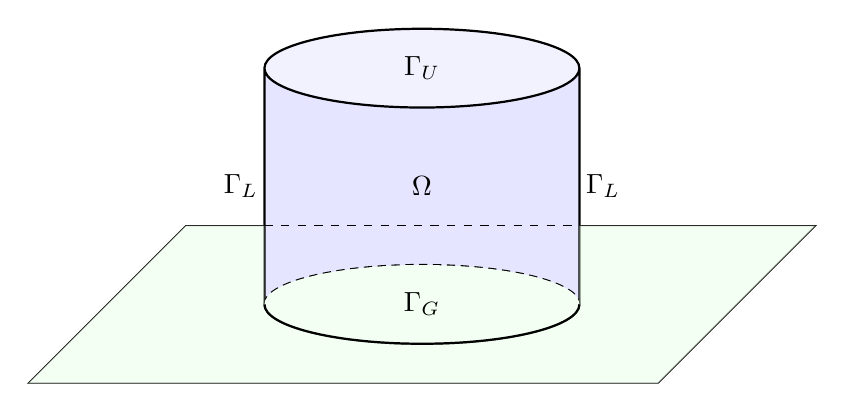
\begin{tikzpicture}
    \fill[color=blue!10] (2,0) -- (2,3) arc (360:180:2cm and 0.5cm) -- (-2,0) arc (180:360:2cm and 0.5cm);
    \fill[color=blue!5] (0,3) circle (2cm and 0.5cm);
    
    \draw[thick] (-2,3) -- (-2,0) arc (180:360:2cm and 0.5cm) -- (2,3) ++ (-2,0) circle (2cm and 0.5cm);
    \draw[densely dashed, thick] (-2,0) arc (180:0:2cm and 0.5cm);
    \draw (-2,1) -- (-3,1) --(-5,-1) -- (3,-1) -- (5,1) -- (2,1);
    \draw[dashed] (-2,1) -- (2,1);
    
    \fill[green!10,opacity=0.5] (-2,0) -- (-2,1) -- (-3,1) -- (-5,-1) -- (3,-1) -- (5,1) -- (2,1) -- (2,0) arc (0:180:2cm and -0.5cm);
    \fill[color=green!5] (0,0) circle (2cm and 0.5cm);
    
    \draw (0,1.5) node {$\Omega$};
    \draw (0,3) node {$\Gamma_U$};
    \draw (0,0) node {$\Gamma_G$};
    \draw (-2.3,1.5) node {$\Gamma_L$};
    \draw (2.3,1.5) node {$\Gamma_L$};
    
    \draw[thick] (2,0) arc (360:180:2cm and 0.5cm);
  \end{tikzpicture}
  \caption{The boundary structure of $\Omega$ for the case of weak solutions}
  \label{structdomaingraphboundaries_weak}
\end{figure}

The boundary conditions to describe the anisotropic system can be summarised as
  
    \begin{equation} \label{ANSC7}
      \begin{split}
        & \mathbf{u}^\epsilon = 0 \text{ on } \Gamma \times (0,T), \\
        & c^\epsilon = 0 \text{ on } ( \Gamma_U \cup \Gamma_L) \times (0,T), \\
        & \partial_2 c^\epsilon = \partial_3 c^\epsilon = 0 \text{ on } \Gamma_G \times (0,T), \quad \partial_1 c^\epsilon = \sigma \in L^2 (0,T; \Gamma_G), \\
      \end{split}
    \end{equation}

while for the hydrostatic case we use
    
    \begin{equation} \label{HNSC7}
      \begin{split} 
        & u_1 = u_2 = u_3 = 0 \text{ on } \Gamma \times (0,T) \\
        & c = 0 \text{ on } ( \Gamma_U \cup \Gamma_L) \times (0,T), \\
        & \partial_2 c = \partial_3 c = 0 \text{ on } \Gamma_G \times (0,T), \partial_1 c \in L^2 L^2 (0,T; \Gamma_G). \\
      \end{split}
    \end{equation}
    
The meaning of $\partial_1 c^\epsilon = \sigma$ above is that we naturally assume $\partial_1 c^\epsilon$ to be equal to some sufficiently regular $\sigma$ function defined on the respective boundary --- this well-known technique is also used for example for the case of modelling wind traction effect on the surface of the ocean.

As we have mentioned it in the introduction, in this case we will work with a more regular ${\mathbf{u}_h}_0 \in H^1$ initial data, so we will directly use the $u_3 = 0$ equality on the boundary instead of the original $u_3 n_3 = 0$ constraint that we had used.
    
We highlight the difference between the boundary conditions of the original, east-north oriented, and the new, downwind matching model for the case of weak solutions.

The difference in the kind of boundary conditions we can "afford" to have on the lower boundary for the concentration comes from the energy inequality. In the east-north-upwards oriented coordinate system we do not have an $\epsilon$ in the diffusion matrix, and thus, having any of the $\partial_i c^\epsilon$ terms different from 0 does not create any problems, not even for an ocean case where $\partial_3 c^\epsilon$ becomes nonzero as well (they are required however to be bounded of course). On the other hand, the downwind matching coordinate system brings in an $\epsilon$ term in front of the $K_1$ diffusion coefficient, which makes the model more sensitive to assigning boundary conditions for $c^\epsilon.$ This means that we can not have anymore the relatively relaxed boundedness requirement for any $\partial_i c^\epsilon$ except for $i=1.$ All other $\partial_2 c^\epsilon, \partial_3 c^\epsilon$ derivatives must be zero on the lower boundary, otherwise they would result in an $(\epsilon - \text{const.})$ negative term appearing in the energy inequality --- for more details see section $\ref{proof}$. This also means that we will consider exclusively the inland domain scenario for the case of this coordinate system.

Finally, the $s^\epsilon$ and $s$ source terms both centred at $\mathbf{x_s}$, with an activation multiplier set to start at time $t_s$. For more details see \cite{pollatmws2019}.

%%% *** WEAK FORMULATION AND MAIN RESULT*** %%%
\subsection{Weak Formulation and Main Result} \label{weakformulationmainresult}

In this section we describe the weak formulation of the merged equations in both the anisotropic and hydrostatic case, and we state our main result.
  
  We need to define the following spaces:
  
  \[ C^{\infty}_\Gamma (\Omega) = \{ \varphi \in C^\infty (\bar{\Omega}); \varphi = 0 \text{ on some neighbourhood of } \Gamma\} \]
  
  \[ H^k_{\Gamma} (\Omega) = \overline{C_\Gamma ^ \infty (\Omega)} ^ {H^k (\Omega)} = \{ v \in H^k(\Omega); v=0 \text{ on } \Gamma \} \]
  
  \[ \mathbf{V} = \{ \mathbf{u} \in  H^1_{\Gamma} (\Omega) \times H^1_{\Gamma} (\Omega) \times H^1_{\Gamma} (\Omega); \nabla \cdot \mathbf{u} = 0 \text{ in } \Omega \} \]
  
  \[ H (\partial_3, \Omega) = \{ v \in L^2(\Omega); \partial_3 v \in L^2 (\Omega)\} \]
  
  \[ H_\Gamma (\partial_3, \Omega) = \overline{C_0 ^\infty (\Omega)}^{H (\partial_3, \Omega)} = \{ v \in H(\partial_3, \Omega); v = 0 \text{ on } \Gamma \} \]
  
  \[ \mathbf{W} = \{ \mathbf{u} \in  H^1_{\Gamma} (\Omega) \times H^1_{\Gamma} (\Omega) \times H_\Gamma (\partial_3, \Omega); \nabla \cdot \mathbf{u} = 0 \text{ in } \Omega \} \]
  
  Then the weak formulation of the hydrostatic system (\ref{HNSC1}) - (\ref{HNSC6}), (\ref{HNSC7}) takes the following form.
  
  \begin{definition} \label{definitionhydrostaticWF}
  
  Find $(\mathbf{u}, c)$ such that $\mathbf{u} = (\mathbf{u}_h, u_3) \in L^2 (0, T; \mathbf{W})$ with $\mathbf{u}_h \in L^\infty (0,T; L^2(\Omega)^2),$ and $c \in L_t^\infty L_x^2$ with $\partial_2 c, \partial_3 c \in L^2_t L^2_x$, such that
  
  \begin{equation}
    \begin{split}
      & \int_0^T \bigg[ -(\mathbf{u}_h, \partial_t \mathbf{\tilde{u}}_h) + (\nabla_\nu \mathbf{u}_h, \nabla_\nu \mathbf{\tilde{u}}_h) - (\mathbf{u}_h, (\mathbf{u} \cdot \nabla) \mathbf{\tilde{u}}_h) + (b(\mathbf{u}_h), \mathbf{\tilde{u}}_h) \bigg ] \diff t \\
      & = - ({\mathbf{u}_h}_0, \mathbf{\tilde{u}}_h(0)) \diff t \label{hydrostaticWF}
    \end{split}
  \end{equation}
  
  and
  
  \begin{equation}
    \begin{split} \nonumber
      &+ \int_0^T \bigg[ -(c, \partial_t \tilde{c}) -(\mathbf{u}c, \nabla \tilde{c}) + K_2 (\partial_2 c, \partial_2 \tilde{c}) + K_3 (\partial_3 c, \partial_3 \tilde{c}) \bigg ] \diff t \\
      & = - (c_0, \tilde{c}(0)) + \int_0^T (s,\tilde{c}) \diff t
    \end{split}
  \end{equation}
  
  for all $(\mathbf{\tilde{u}}, \tilde{c})$ with $\mathbf{\tilde{u}} = (\mathbf{\tilde{u}}_h, \tilde{u}_3) \in H^1 (0,T, \mathbf{W})$, with $\mathbf{\tilde{u}}_h (T) = 0$ and $\partial_3 \mathbf{\tilde{u}}_h \in L^\infty (0, T; L^3 (\Omega)^2)$ and $\tilde{c}$ with $\tilde{c} \in L^2 (0,T, H^3_{\Gamma} (\Omega))$, $\tilde{c} \in H^1 (0,T, L^2)$, $\tilde{c} (T) = 0$. 
  
  \end{definition}
  
  Giving definition to the weak formulation of the anisotropic system we underline the importance of the spaces we use here --- they create a sort of in-between point for classical weak solutions and Leray-Hopf weak solutions in the sense that the concentration function does not need to be weakly continuous, but the velocity part of the solution is set to be in $C_w.$ This represents a space construction that is both minimal and corresponds to the requirements of the proof detailed later.

 \begin{definition} \label{definitionanisotropicWF}
  
  Find $\mathbf{u}^\epsilon = (\mathbf{u}_h, u^\epsilon_3) \in L^2 (0,T ; \mathbf{V}) \cap C_w (0, T; L^2 (\Omega)^3)$ and $c^\epsilon \in L^\infty (0,T; L^2(\Omega)) \cap L^2 (0,T; H^1(\Omega))$, such that
  
  \begin{equation}
    \begin{split}
      & \int_0^T \bigg [ -(\mathbf{u}^\epsilon_h, \partial_t \mathbf{\tilde{u}}_h) + (\nabla_\nu \mathbf{u}^\epsilon_h, \nabla_\nu \mathbf{\tilde{u}}_h) - (\mathbf{u}^\epsilon_h, (\mathbf{u}^\epsilon \cdot \nabla) \mathbf{\tilde{u}}_h) + (b(\mathbf{u}^\epsilon_h), \mathbf{\tilde{u}}_h) \bigg ] \diff t \\
      & + \epsilon \beta \int_0 ^ T \big [ (u_3 ^\epsilon, \tilde{u}_1) - (u_1^\epsilon, \tilde{u}_3) \big ] \diff t + \epsilon \alpha \int_0 ^ T \big [ (u_2 ^\epsilon, \tilde{u}_3) - (u_3^\epsilon, \tilde{u}_2) \big ] \diff t\\
      & + \epsilon^2 \int _0 ^ T \big [ -(u_3^\epsilon, \partial_t \tilde{u}_3) +(\mathbf{u}^\epsilon \cdot \nabla u_3 ^ \epsilon, \tilde{u}_3) + (\nabla_\nu u_3^\epsilon, \nabla_\nu \tilde{u}_3) \big ] \diff t \\
      & = - ({\mathbf{u}^\epsilon_h}_0, \mathbf{\tilde{u}}_h(0)) - \epsilon^2 ({u^\epsilon_3}_0, \tilde{u}_3 (0)) \diff t \raisetag{20pt} \label{anisotropicWF}
    \end{split}
  \end{equation}
  
    and
  
    \begin{equation}
    \begin{split} \nonumber
      & \int_0^T \bigg [ -(c^\epsilon, \partial_t \tilde{c}) -(\mathbf{u}^\epsilon c^\epsilon, \nabla \tilde{c}) + \epsilon K_1 (\partial_1 c^\epsilon, \partial_1 \tilde{c}) - \epsilon K_1 \sigma \big[\tilde{c} \big] _{\Gamma_G} \\
      & + K_2 (\partial_2 c^\epsilon, \partial_2 \tilde{c}) + K_3 (\partial_3 c^\epsilon, \partial_3 \tilde{c}) \bigg ] \diff t \\
      & =  - (c_0, \tilde{c} (0)) + \int_0^T (s^\epsilon,\tilde{c}) \diff t
    \end{split}
  \end{equation}
  
  for all $\mathbf{\tilde{u}} = (\mathbf{\tilde{u}}_h, \tilde{u}_3) \in H^1 (0,T;\mathbf{V})$ with $\mathbf{\tilde{u}}(T) = 0$ and $\tilde{c}$ such that $\tilde{c} \in H^1 (0,T, H^3_{\Gamma} (\Omega))$ and $\tilde{c} (T) = 0$.
  
  \end{definition}

The main theorem of this paper is analogous to our previous result stated for the case of the geophysical frame, but we highlight the difference that here we use the initial data ${\mathbf{u}_h}_0 \in H^1,$ while for the case of the geophysical frame an $L^2$ initial velocity was sufficient.

Now we are ready to state the main theorem of this section.

\begin{theorem} \label{maintheoremWEAK}
  Let ${\mathbf{u}_h}_0$ $\in$ $H^1 (\Omega)$, ${u_3}_0 \in L^2(\Omega)$ with $\nabla \cdot \mathbf{u}_0 = 0, \mathbf{u}_0 = 0$ on $\partial \Omega$; let $c_0 \in$ $L^2 (\Omega)$, $c_0 = 0$ on $ \partial \Omega$, and assume that the boundary conditions (\ref{ANSC7}) hold; then as the aspect ratio $\epsilon$ tends to zero, any weak solution $(\mathbf{u}^\epsilon, c^\epsilon)$ of the anisotropic equations (\ref{ANSC1}) - (\ref{ANSC6}) converges to a weak solution $(\mathbf{u}, c)$ of the hydrostatic equations of the polluted atmosphere (\ref{HNSC1}) - (\ref{HNSC6}).
\end{theorem}
  
%%% *** PROOF *** %%%
\subsection{Proof of the main theorem} \label{proof}

This section is dedicated to the verification of Theorem \ref{maintheoremWEAK}. Structurally we follow a similar chain of thought as in our previous paper --- until the point where the proof diverges reaching the weak convergence of the nonlinear term $u_3^\epsilon C^\epsilon,$ where in this case we can not benefit from an $H^1$-regular concentration function. In more detail, we begin by calculating the energy inequality and collect the a priori estimates that derive from it, then verify the less problematic weak convergence results. Finally we elaborate the steps that bring the convergence of the $u_3^\epsilon C^\epsilon$ term to a closure. The main idea here is to temporarily ignore the $C^\epsilon$ function and prove a strong convergence result considering only the velocity functions. Throughout this step we go beyond the weak solutions quality and show that we are working with strong solutions. In this new setting with more favourable regularities we can prove the convergence result we need, and eventually return to the frame of weak solutions where we can merge back together the velocity and concentration functions into a unified solution.

  \subsubsection{Energy inequality and a priori estimates}
  
  Calculating the energy inequality for the anisotropic system, we obtain that for a.e. $t \in [0,T]$ the following holds:
  
  \begin{equation}
    \begin{split}  
    & \frac{1}{2} (\norm{\mathbf{u}_h^\epsilon (t)}_{L^2}^2 + \epsilon ^ 2 \norm{u_3^\epsilon (t)}_{L^2}^2 + \norm{C^\epsilon (t)}_{L^2}^2) + \int_0 ^ t \big[ \norm{\nabla_\nu \mathbf{u}_h^\epsilon}_{L^2}^2 + \epsilon ^ 2 \norm{\nabla_\nu u_3^\epsilon}_{L^2}^2  \big] \diff \tau \\
    & + \int_0 ^ t  \big [ \epsilon K_1 \norm{\partial_1 C^\epsilon}_{L^2}^2  + K_2 \norm{\partial_2 C^\epsilon}_{L^2}^2 + K_3 \norm{\partial_3 C^\epsilon}_{L^2}^2 \big ] d \tau \\
    & \leq \int_0^t (S^\epsilon,C^\epsilon) \diff \tau + \frac{1}{2} (\norm{\mathbf{u}_h^\epsilon (0)}_{L^2}^2 + \epsilon ^ 2 \norm{u_3^\epsilon (0)}_{L^2}^2 + \norm{C^\epsilon_0}_{L^2}^2) \\
    & + \int _ 0 ^ t \epsilon K_1 \langle \partial_1 C^\epsilon, C^\epsilon \rangle_{\Gamma_G} \diff \tau \raisetag{70pt} \label{energyIEQ}
    \end{split}
  \end{equation}
  
  Using standard techniques, the generalised Young inequality with a $\zeta > 0$ constant, the H\"older inequality and the Trace Theorem, (\ref{energyIEQ}) takes the final form

  \begin{equation}
    \begin{split}  
    & \frac{1}{2} (\norm{\mathbf{u}_h^\epsilon (t)}_{L^2}^2 + \epsilon ^ 2 \norm{u_3^\epsilon (t)}_{L^2}^2 + \norm{C^\epsilon (t)}_{L^2}^2) + \int_0 ^ t \big [\norm{\nabla_\nu \mathbf{u}_h^\epsilon}_{L^2}^2 + \epsilon ^ 2 \norm{\nabla_\nu u_3^\epsilon}_{L^2}^2 \big ] \diff \tau \\
    & + \int_0 ^ t \bigg[ (\epsilon K_1 - \zeta \frac{\epsilon}{2} K_1 c_T (c_S + 1)) \norm{\partial_1 C^\epsilon}_{L^2}^2  + (K_2 - \zeta \frac{\epsilon}{2} K_1 c_T (c_S + 1)) \norm{\partial_2 C^\epsilon}_{L^2}^2 \\
    & + (K_3 - \zeta \frac{\epsilon}{2} K_1 c_T (c_S + 1)) \norm{\partial_3 C^\epsilon}_{L^2}^2 \bigg] \diff \tau \\
    & \leq \frac{1}{\zeta} K_1 \frac{\epsilon}{2} \int_0 ^ t \norm{\partial_1 C^\epsilon}^2 _{L^2 (\Gamma_G)} + \frac{1}{2} (\norm{\mathbf{u}_h^\epsilon (0)}_{L^2}^2 + \epsilon ^ 2 \norm{u_3^\epsilon (0)}_{L^2}^2 + \norm{C^\epsilon (0)}_{L^2}^2) \\
    & + \int_0^t (S^\epsilon,C^\epsilon) \diff \tau, \raisetag{20pt} \label{finalformEIEQ}
    \end{split}
  \end{equation}
  
  where $c_T$ and $c_S$ are the constants provided by the Trace Theorem and Sobolev embeddings. The boundary term is bounded because of the a priori assumptions made on the boundary conditions.
    
  The right-hand side of the energy inequality is now apparently bounded, and it is easy to see that the coefficients of the pollution terms on the left-hand side are positive, since the $\zeta$ constant of the generalised Young inequality can be freely chosen in a way such that the requirements $\epsilon K_1 (1 - \zeta \frac{1}{2} c_T (c_S + 1)) > 0, (K_2 - \zeta \frac{\epsilon}{2} K_1 c_T (c_S + 1)) > 0, (K_3 - \zeta \frac{\epsilon}{2} K_1 c_T (c_S + 1)) > 0 $ are all satisfied.
  
  We note that the most significant difference in this new form of the energy inequality (\ref{finalformEIEQ}) is having $\sqrt{\epsilon} \partial_1 C^\epsilon$ in the place of $\partial_1 C^\epsilon,$ which is what we had for the case of the geophysical coordinate system. It leads to the disappearance of the $H^1$ regularity of $C^\epsilon,$ and thus we don't have the strong convergence feature of the concentration function anymore --- which was of key importance for proving the weak convergence of a nonlinear term in the case of the classical geophysical frame.
  
  This form of the energy inequality also shows why we need the $\partial_2 C^\epsilon, \partial_3 C^\epsilon$ terms to vanish on the boundary. Otherwise, using the Trace Theorem on these boundary terms would contribute to the appearance of negative, $\epsilon$-free terms in the coefficient of $\norm{\partial_1 C^\epsilon}_{L^2}^2,$ which would undermine the structure of the energy inequality.
  
  From the final form of the energy inequality (\ref{finalformEIEQ}) we obtain uniform a priori estimates that we summarise in the following proposition.
  
  \begin{prop} \label{aprioriprop}
    Let $u^\epsilon_1, u^\epsilon_2, u^\epsilon_3$ and $C^\epsilon$ be the weak solutions of the system (\ref{ANSC1}) - (\ref{ANSC5}) in the sense of Definition \ref{definitionanisotropicWF}. Then it holds,
    
    \begin{align}
      & u^\epsilon_1, u^\epsilon_2, \epsilon u^\epsilon_3, C^\epsilon & \quad & \text{are bounded in $L^\infty (0,T; L^2(\Omega)),$} \label{proposition1} \\
      & u^\epsilon_3 & \quad & \text{is bounded in $L^2 (0,T; L^2(\Omega)),$} \label{propositionExtra} \\
      & u^\epsilon_1, u^\epsilon_2, \epsilon u^\epsilon_3 & \quad & \text{are bounded in $L^2(0,T; H^1(\Omega)),$} \label{proposition2} \\
      & \sqrt{\epsilon} \partial_1 C^\epsilon, \partial_2 C^\epsilon, \partial_3 C^\epsilon & \quad & \text{are bounded in $L^2(0,T;L^2(\Omega)).$} \label{proposition3}
    \end{align}
    
  \end{prop}
  
  For the details of the proof see \cite{pollatmws2019}.
  
    \subsubsection{Weak convergence - Part 1.}
  
  The \textit{i)} a priori estimates, \textit{ii)} the convergence of the linear terms and also, \textit{iii)} the convergence of the nonlinear terms with the exception of $u_3^\epsilon C^\epsilon$ can be proved analogously as in our previous paper --- the proofs of these properties are not affected by the changes induced by choosing to use the downwind matching coordinate system. Hence, for completeness we will describe the main steps leading up to obtaining these results, but we will skip the details. For technical or specific issues see \cite{azerad2001mathematical} and \cite{pollatmws2019}.
  
  As a consequence of Proposition \ref{aprioriprop}, up to subsequences still denoted by the same way, we have the following weak convergence results.
  
    \begin{align} 
    &  \mathbf{u}_h^\epsilon \rightharpoonup \mathbf{u}_h &\quad & \text{weakly in $L_t^\infty L_x^2 \cap L_t^2 H_x^1$,} \label{WeakConvUHEps} \\
    &  \epsilon^2 u_3^\epsilon \to 0 &\quad & \text{strongly in $L_t^\infty L_x^2 \cap L_t^2 H_x^1$,} \label{WeakConvU3Eps} \\ 
    & u_3^\epsilon \rightharpoonup u_3  &\quad & \text{weakly in $L_t^2 L_x^2$,} \label{WeakConvU3NoEps} \\
    & C^\epsilon \rightharpoonup C &\quad & \text{weakly in $L_t^\infty L_x^2$,} \label{WeakConvCEps1} \\
    & \partial_2 C^\epsilon \rightharpoonup \partial_2 C &\quad & \text{weakly in $L_t^2 L_x^2$,} \label{WeakConvCEps2} \\
    & \partial_3 C^\epsilon \rightharpoonup \partial_3 C &\quad & \text{weakly in $L_t^2 L_x^2$,} \label{WeakConvCEps3} \\
    & \sqrt{\epsilon} \partial_1 C^\epsilon \rightharpoonup e &\quad & \text{weakly for some limit element $e$ in $L_t^2 L_x^2$.} \label{WeakConvCEps4}
  \end{align} 
  
  In order to conclude the proof of Theorem \ref{maintheorem} we pass to the limit in the weak formulation (\ref{anisotropicWF}). Taking the limit for the linear terms can be done in a standard way using the previously obtained results.
   Concerning the nonlinear velocity terms (i.e. nonlinear terms that do not include the concentration function), the convergence can be shown applying a generalisation of the classical translation criterium of Riesz-Frechet-Kolmogorov which enables us to get strong convergence for the horizontal velocities. This is achieved by establishing a bound for the perturbation of $\mathbf{u}_h$ of the form $\norm{\tau_\pi \mathbf{u}_h - \mathbf{u}_h}_{L^2(0,T-\pi, {H^2}^*)} \leq \lambda(\pi) + \mu(\epsilon),$ where $\lambda$ and $\mu$ are appropriate functions with their limits vanishing at zero, and $\tau_\pi \mathbf{u}_h = \mathbf{u}_h (t+\pi) $. After obtaining strong convergence for $\mathbf{u}_h,$ the proof of the convergence for these nonlinear terms can be closed by applying basic interpolation techniques and the generalised H\"older inequality. 
  Finally, as for the concentration-including nonlinear terms, we have the convergence of $(u_i C^\epsilon, \partial_i \tilde{C})$ for $i=1,2,$ since as we mentioned before, we have the strong convergence of the horizontal velocities --- while in the case of $i=3$ this property does not hold for $u_3$ and from the energy bound we do not have more than the weak convergence of $C^\epsilon$. Because of its complexity we handle this specific nonlinear compound product term in the next section.
  
  \subsubsection{Weak convergence - Part 2.}
  
  As we mentioned before, the cornerstone idea for obtaining the convergence of the remaining product term $u_3^\epsilon C^\epsilon$ is to exploit the $H^1$ regularity of the initial horizontal velocity. Indeed, given an $H^1$ initial data for $\mathbf{u}_h,$ according to the theory developed in \cite{cao2007global}, there exists a unique global strong solution for the primitive equations $(\ref{HNSC1})$ - $(\ref{HNSC4}).$ We recall here this result (for more details see \cite{cao2007global}).
  
  \begin{theorem} \label{PE3DWellPosedness}
    Let ${\mathbf{u}_h}_0 \in H^1(\Omega).$ Then there exists a unique strong solution $\mathbf{u}_h$ of the reformulated Primitive Equations $(\ref{HNSC1})$ - $(\ref{HNSC4})$, $(\ref{HNSC6})$ such that $$\mathbf{u}_h \in C([0, \infty), H^1(\Omega)) \cap L^2_{loc}([0, \infty), H^2(\Omega))$$ and $$\partial_t \mathbf{u}_h \in L^2_{loc} ([0,\infty), L^2(\Omega)).$$
  \end{theorem}
  
  In more detail, we have the following regularities for the strong solution of the primitive equations for the case of an $H^1$ initial data:
  
  \begin{corollary} \label{StrongSolPE_boundedness}
  
    Let $(\mathbf{u}_h,u_3)$ be the the unique global strong solution to the primitive equations (\ref{HNSC1}) - (\ref{HNSC4}) with an initial data ${\mathbf{u}_h}_0 \in H^1(\Omega).$ Then we have the following boundedness result:
    
    $$ \sup_{0 \leq t < \infty} \norm{\mathbf{u}_h}_{H^1}^2 (t) + \int_0^\infty \norm{\nabla \mathbf{u}_h}_{H^1}^2 \diff t \leq C(\norm{{\mathbf{u}_h}_0}_{H^1}, \Gamma_G).$$
  
  \end{corollary}
  
  This is a direct consequence of Theorem \ref{PE3DWellPosedness}, but for completeness we also mention that for the simpler case of a periodic domain it has also been verified in \cite{li2019primitive}, where the proof becomes more straightforward thanks to the structure of the domain.
  
  The result of Corollary \ref{StrongSolPE_boundedness} on the strong solutions of the primitive equations will be indispensable later, as we will use these strong solution functions for testing the scaled Navier-Stokes equations.
  
  The following part of the proof is dedicated to verifying the strong convergence of $u_3^\epsilon,$ and is based on the idea of \cite{li2019primitive} --- our scenario is different however in that \textit{a)} first of all our domain is bounded, while the domain the authors of \cite{li2019primitive} consider is periodic, \textit{b)} we do not assume zero-averaged functions, and finally \textit{c)} in our case the Coriolis terms are incorporated to the model as well. Our strategy in providing the proof is to give a self-contained result that describes all the steps that build up the verification process, but we elaborate in more detail where the above mentioned \textit{a), b), c)} points have a tangible effect. Some technical details that are identical to those in \cite{li2019primitive} will be skipped.

Another structural difference we need to underline in connection with the proof is that instead of using the $[-1,1]$ set to represent the $\epsilon$-free vertical domain (i.e. the $\Gamma_L$ section), we use $[0,1],$ without assuming the vertical velocity function $u_3^\epsilon$ to be odd with respect to $z.$ The vertical section is commonly set to $[-1,1],$ or equivalently, to $[-a,a]$ in works that use the periodical domain scenario, see also \cite{cao2016global}, \cite{cao2017global}. In our case however we use a bounded domain without the assuming a symmetry line in the vertical midpoint --- thus we work with the $[0,1]$ set as the vertical domain. As a consequence, the Ladyzhenskaya-type inequality presented in different versions in \cite{cao2003global} and \cite{li2019primitive} will be used here in the following form:

\begin{lemma}\label{LadyzhenskayatypeIEQ}

  The inequalities
  
  \begin{equation}\nonumber
    \begin{split}
      & \int_{\Gamma_G} \bigg ( \int_0^1 f(x,y,z) \diff z \bigg) \bigg ( \int_0^1 g(x,y,z) h(x,y,z) \diff z \bigg ) \diff x \diff y \\
      & \leq C \norm{f}_2^{1/2} \big ( \norm{f}_2^{1/2} + \norm{\nabla_h f}_2^{1/2} \big ) \norm{g}_2 \norm{h}_2^{1/2} \big (\norm{h}_2^{1/2} + \norm{\nabla_h h}_2^{1/2} \big ),
    \end{split}
  \end{equation}
  
  and
  
  \begin{equation}\nonumber
    \begin{split}
      & \int_{\Gamma_G} \bigg ( \int_0^1 f(x,y,z) \diff z \bigg) \bigg ( \int_0^1 g(x,y,z) h(x,y,z) \diff z \bigg ) \diff x \diff y \\
      & \leq C \norm{f}_2 \norm{g}_2^{1/2} \big ( \norm{g}_2^{1/2} + \norm{\nabla_h g}_2^{1/2} \big ) \norm{h}_2^{1/2} \big (\norm{h}_2^{1/2} + \norm{\nabla_h h}_2^{1/2} \big )
    \end{split}
  \end{equation}
  
  hold true for any $f,g,h$ set of functions such that the right-hand sides make sense and are finite. Here $C$ is a positive constant depending only on $\Gamma_G.$

\end{lemma}

Note that this lemma simply states the inequality for the complete domain even in the version in \cite{li2019primitive}, not assuming an odd $u_3^\epsilon$ function or a $z$-symmetrical vertical structure of $\Omega$.
  
The main idea in order to prove the strong convergence of $u^\epsilon_3$ lies in establishing a bound of $O(\epsilon^a)$ for some $a>0$ for the difference $$(\mathbf{U}_h^\epsilon, U_3^\epsilon): = (\mathbf{u}_h^\epsilon - \mathbf{u}_h, u_3^\epsilon - u_3).$$ This will be achieved by using the strong solution $(\mathbf{u}_h,u_3)$ as a test function in the weak formulation's integral identity $(\ref{anisotropicWF})$. Following this method we arrive to

\begin{prop} \label{propIdentity}

Let $(\mathbf{u}_h^\epsilon, u_3^\epsilon)$ and $(\mathbf{u}_h,u_3)$ be the solutions of (\ref{ANSC1}) - (\ref{ANSC4}) and (\ref{HNSC1}) - (\ref{HNSC4}), respectively, with initial data $({\mathbf{u}_h}_0, {u_3}_0),$ where ${\mathbf{u}_h}_0 \in H^1(\Omega)$ and ${u_3}_0 = - \int_0^z \nabla_h \cdot {\mathbf{u}_h}_0 \diff z'.$ Then we have the following integral identity:

\begin{equation} \label{integralIdentity_prop}
  \begin{split}
    & - \frac{\epsilon^2}{2} \norm{u_3(t)}_2^2 + \bigg ( (\mathbf{u}_h^\epsilon \cdot \mathbf{u}_h + \epsilon^2 u_3^\epsilon u_3) \diff x \diff y \diff z  \bigg ) (t) \\
    & + \int_{Q_t} (-\mathbf{u}_h^\epsilon \cdot \partial_t \mathbf{u}_h + \nabla \mathbf{u}_h^\epsilon : \nabla \mathbf{u}_h + \epsilon^2 \nabla u_3^\epsilon \cdot \nabla u_3) \diff x \diff y \diff z \diff s \\
    & = \frac{\epsilon^2}{2} \norm{{u_3}_0}_2^2 + \norm{{\mathbf{u}_h}_0}_2^2 + \epsilon^2 \int_{Q_t} \bigg ( \int_0^z \partial_t \mathbf{u}_h \diff z' \bigg ) \cdot \nabla_h U_3^\epsilon \diff x \diff y \diff z \diff s \\
    & - \int_{Q_t} [(\mathbf{u}^\epsilon \cdot \nabla) \mathbf{u}_h^\epsilon \cdot \mathbf{u}_h + \epsilon^2 \mathbf{u}^\epsilon \cdot \nabla u_3^\epsilon u_3] \diff x \diff y \diff z \diff s \\
    & + \int_{Q_t}  ( \gamma u_2^\epsilon u_1 - \epsilon \beta u_3^\epsilon u_1 + \alpha \epsilon u_3^\epsilon u_2 - \gamma u_1^\epsilon u_2 - \epsilon \alpha u^\epsilon_2 u_3 + \epsilon \beta u_1^\epsilon u_3)
  \end{split}
\end{equation}

for any $t \in [0, \infty),$ where $Q_t = \Omega \times (0,t).$

\end{prop}

\begin{proof}

We recall the definition of weak solution for the scaled Navier-Stokes equations:

\begin{equation} \label{WFreminder}
  \begin{split}
    & \int_Q [ - (\mathbf{u}_h^\epsilon \cdot \partial_t \tilde{\mathbf{u}}_h + \epsilon^2 u_3^\epsilon \partial_t \tilde{u}_3) +( (\mathbf{u}^\epsilon \cdot \nabla) \mathbf{u}_h^\epsilon \cdot \tilde{\mathbf{u}}_h + \epsilon^2 \mathbf{u}^\epsilon \cdot \nabla u_3^\epsilon \tilde{u}_3 ) + \nabla \mathbf{u}_h^\epsilon : \nabla \tilde{\mathbf{u}}_h \\
    & + \epsilon^2 \nabla u_3^\epsilon \cdot \nabla \tilde{u}_3 ] \diff x \diff y \diff z \diff t = \int_Q ({\mathbf{u}_h}_0 \cdot \tilde{\mathbf{u}}_h (\cdot , 0) + \epsilon^2 {u_3}_0 \tilde{u}_3 (\cdot , 0)) \diff x \diff y \diff z \\
    & + \int_Q  \gamma u_2^\epsilon \tilde{u}_1 - \epsilon \beta u_3^\epsilon \tilde{u}_1 + \alpha \epsilon u_3^\epsilon \tilde{u}_2 - \gamma u_1^\epsilon \tilde{u}_2 - \epsilon \alpha u_2^\epsilon \tilde{u}_3 + \epsilon \beta u_1^\epsilon \tilde{u}_3
  \end{split}
\end{equation}

for any $\tilde{\mathbf{u}} = (\tilde{\mathbf{u}}_h, \tilde{u}_3) \in H^1 (0,T;\mathbf{V})$ with $\tilde{\mathbf{u}}(T) = 0.$

Now, let's define $\chi \in C_0^\infty ([0, \infty))$ with $0 \leq \chi \leq 1$ and $\chi (0) = 1$ and set $\tilde{\mathbf{u}} = (\mathbf{u}_h,u_3) \chi (t).$ By using the density argument it is valid to choose this $\tilde{\mathbf{u}}$ function as a testing function as long as all the integral terms remain well-defined in $(\ref{WFreminder}),$ which we verify in the following.

It is important to highlight at this point that since we are not restricted to zero-averaged functions and we are not on a periodic domain, we need to pay special attention when verifying boundedness results using the Poincar\'e inequality. Note that as the value of the velocity functions are defined to be zero on the boundary, any first-order estimate of the type $\norm{\mathbf{u}_h^\epsilon} \leq \norm{\nabla \mathbf{u}_h^\epsilon}$ is valid (i.e. to estimate a function by its gradient), using the zero-trace version of the Poincar\'e inequality for functions in $W^{1,2}_0.$ However, since it is only the value of the functions that vanishes on the boundary, but not their derivatives, higher order estimates such as passing from $\norm{\nabla \mathbf{u}_h^\epsilon}$ to $\norm{\Delta \mathbf{u}_h^\epsilon}$ in the process of constructing an upper bound can not be applied in general. Which is why, for example, the estimate of the the term below is rather involved as follows:

\begin{equation}
  \begin{split}
    & \int_Q \abs{\mathbf{u}^\epsilon} \abs{\nabla u_3^\epsilon} \abs{u_3} \chi \diff x \diff y \diff z \\
    & \leq  \int_0 ^ T \int_{\Gamma_G} \bigg ( \int_0^1 \abs{\mathbf{u}^\epsilon} \abs{\nabla u_3^\epsilon} \diff z \int_0^1 \abs{\nabla_h \mathbf{u}_h} \diff z \bigg ) \diff x \diff y \diff t \\
    & \leq C \int_0^T \norm{\mathbf{u}^\epsilon}_2^{1/2} \norm{\nabla \mathbf{u}^\epsilon}_2^{1/2} \norm{\nabla u_3^\epsilon}_2 \norm{\nabla_h \mathbf{u}_h}_2^{1/2} (\norm{\nabla_h \mathbf{u}_h}_2^{1/2} + \norm{\Delta \mathbf{u}_h}_2^{1/2}) \diff t \\
    & \leq C \sup_{0 \leq t \leq T} \bigg( \norm{\mathbf{u}^\epsilon}_2^{1/2} \norm{\nabla \mathbf{u}_h}_2^{1/2} \bigg) \bigg( \int_0^T \norm{\nabla \mathbf{u}^\epsilon}^2_2 \diff t \bigg)^{1/4} \bigg ( \int_0^T \norm{\nabla u_3^\epsilon}_2^2 \diff t \bigg)^{1/2} \\
    & \times \bigg ( \int_0^T \norm{\Delta \mathbf{u}_h}_2^2 \diff t \bigg )^{1/4} \\
    & + C \sup_{0 \leq t \leq T} \bigg( \norm{\mathbf{u}^\epsilon}_2^{1/2} \norm{\nabla \mathbf{u}_h}_2 \bigg) \bigg( \int_0^T \norm{\nabla \mathbf{u}^\epsilon}_2 \diff t \bigg)^{1/2} \bigg ( \int_0^T \norm{\nabla u_3^\epsilon}_2^2 \diff t \bigg)^{1/2}.\raisetag{60pt}
  \end{split}
\end{equation}

The validity of the remaining integral terms are not affected by the boundary change and they are guaranteed by the regularities of the respective solution functions and using basic inequalities. For completeness we remark that the more delicate and problematic terms -- i.e. the terms where the testing function is defined via the less regular $u_3$ vertical velocity -- are still well-defined. This can be verified firstly by rewriting the $\int_Q u^\epsilon_3 \partial_t \tilde{u}_3$ term as

$$ \int_Q u^\epsilon_3 \partial_t (u_3 \chi) \diff x \diff y \diff z \diff t = \int_0^\infty \langle \partial_t (u_3 \chi), u^\epsilon_3 \rangle _ {H^{-1} \times H^1} \diff t.$$

The validity of the integral term can be shown using this modified form pointing out that $\partial_t \mathbf{u}_h$ is in $L^2_{loc} ([0,\infty), L^2(\Omega))$ because of Theorem $\ref{PE3DWellPosedness}$, and as a consequence $\partial_t u_3$ has an $H^{-1}$ space regularity (using the divergence-free condition).

On the other hand, the $ \int_Q \nabla u^\epsilon_3 : \nabla (u_3 \chi) $ term is well-defined since $u_3$ as a strong solution has $H^1$ space regularity, and the same holds for the weak solution $u^\epsilon_3.$

Now we are justified to take $\tilde{\mathbf{u}}$ as a test function, and thus, rewriting some of the integral terms in $(\ref{WFreminder})$ in a more convenient form, we have

\begin{equation} \label{rewrittenform}
  \begin{split}
    & \int_Q (- \mathbf{u}_h^\epsilon \cdot \partial_t \mathbf{u}_h + \nabla \mathbf{u}_h^\epsilon : \nabla \mathbf{u}_h + \epsilon^2 \nabla u_3^\epsilon \cdot \nabla u_3) \chi \diff x \diff y \diff z \diff t \\
    & - \epsilon^2 \int_0^\infty \langle \partial_t u_3 , u_3^\epsilon \rangle _{H^{-1} \times H^1} \chi \diff t - \int_Q (\mathbf{u}_h^\epsilon \cdot \mathbf{u}_h + \epsilon^2 u_3^\epsilon u_3) \chi' \diff x \diff y \diff z \diff t \\
    & = - \int_Q [(\mathbf{u}^\epsilon \cdot \nabla) \mathbf{u}_h^\epsilon \cdot \mathbf{u}_h + \epsilon^2 \mathbf{u}^\epsilon \cdot \nabla u_3^\epsilon u_3] \chi \diff x \diff y \diff z \diff t + \norm{{\mathbf{u}_h}_0}_2^2 + \epsilon^2 \norm{{u_3}_0}_2^2 \\
    & + \int_Q  ( \gamma u_2^\epsilon u_1 - \epsilon \beta u_3^\epsilon u_1 + \alpha \epsilon u_3^\epsilon u_2 - \gamma u_1^\epsilon u_2 - \epsilon \alpha u^\epsilon_2 u_3 + \epsilon \beta u_1^\epsilon u_3) \chi,\raisetag{80pt}
  \end{split}
\end{equation}

for any $\chi \in C^\infty_0 ([0,\infty)),$ with $0 \leq \chi \leq 1$ and $\chi (0) = 1.$

Since the estimate $(\ref{integralIdentity_prop})$ is localised in time, we take an arbitrary $t_0 \in (0, \infty)$ and a sufficiently small positive $\delta \in (0, t_0).$ Choose a cut-off function with the properties $\chi_\delta \in C^\infty_0 [0,t_0),$ such that $\chi_\delta \equiv 1$ on $[0, t_0 -\delta], 0 \leq \chi_\delta \leq 1$ on $[t_0 - \delta, t_0 )$ and $\abs{\chi_\delta '} \leq \frac{2}{\delta}$ on $[0, t_0).$ Now, taking $\chi = \chi_\delta$ in $(\ref{rewrittenform})$ as $\delta \to 0,$ one can arrive to the desired equality after performing the calculations for passing to the limit. It is easy to see that because of the velocities vanishing on the boundaries, the technical details remain uneffected, even though we are not on a periodic domain.

In more detail, the term $ \langle \partial_t u_3, u_3^\epsilon \rangle$ now takes the form 

\begin{equation}
  \begin{split}
    & \langle \partial_t u_3, u_3^\epsilon \rangle = - \bigg \langle \nabla_h \cdot \bigg ( \int_0^z \partial_t \mathbf{u}_h \diff z' \bigg ) , u_3^\epsilon \bigg \rangle \\
    & = - \int_{\partial \Omega} \bigg ( \int_0^z \partial_t \mathbf{u}_h \diff z' \bigg ) u_3^\epsilon \mathbf{n}_h + \int_\Omega \bigg ( \int_0^z \partial_t \mathbf{u}_h \diff z' \bigg) \cdot \nabla_h u_3^\epsilon \diff x \diff y \diff z,
  \end{split}
\end{equation}

where $\mathbf{n}_h$ is the horizontal component of the outward facing normal vector on the $\partial \Omega$ boundary.
    
By using that $u_3^\epsilon = 0$ on $\partial \Omega$ we arrive easily to the more simple
    
$$ \langle \partial_t u_3, u_3^\epsilon \rangle  = \int_\Omega \bigg ( \int_0^z \partial_t \mathbf{u}_h \diff z' \bigg) \cdot \nabla_h u_3^\epsilon \diff x \diff y \diff z,$$
     
which is the form one would have on a periodic domain. Similarly, 
     
$$ \langle \partial_t u_3, u_3^\epsilon - u_3 \rangle = \int_\Omega \bigg ( \int_0^z \partial_t \mathbf{u}_h \diff z' \bigg) \cdot \nabla_h (u_3^\epsilon - u_3),$$ as the boundary term $$\int_{\partial \Omega} \bigg ( \int_0^z \partial_t \mathbf{u}_h \diff z' \bigg ) (u_3^\epsilon - u_3) \mathbf{n}_h$$ becomes zero, since we have $u_3 = 0, u_3^\epsilon = 0$ on $\Gamma.$ 

After some technical details that we omit here we eventually obtain

\begin{equation}
  \begin{split}
    & - \frac{\epsilon^2}{2} \norm{u_3(t_0)}_2^2 + \bigg ( (\mathbf{u}_h^\epsilon \cdot \mathbf{u}_h + \epsilon^2 u_3^\epsilon u_3) \diff x \diff y \diff z  \bigg ) (t_0) \\
    & + \int_{Q_{t_0}} (-\mathbf{u}_h^\epsilon \cdot \partial_t \mathbf{u}_h + \nabla \mathbf{u}_h^\epsilon : \nabla \mathbf{u}_h + \epsilon^2 \nabla u_3^\epsilon \cdot \nabla u_3) \diff x \diff y \diff z \diff t \\
    & = \frac{\epsilon^2}{2} \norm{{u_3}_0}_2^2 + \norm{{\mathbf{u}_h}_0}_2^2 + \epsilon^2 \int_{Q_{t_0}} \bigg ( \int_0^z \partial_t \mathbf{u}_h \diff z' \bigg ) \cdot \nabla_h U_3^\epsilon \diff x \diff y \diff z \diff t \\
    & - \int_{Q_{t_0}} [(\mathbf{u}^\epsilon \cdot \nabla) \mathbf{u}_h^\epsilon \cdot \mathbf{u}_h + \epsilon^2 \mathbf{u}^\epsilon \cdot \nabla u_3^\epsilon u_3] \diff x \diff y \diff z \diff t \\
    & + \int_{Q_{t_0}}  ( \gamma u_2^\epsilon u_1 - \epsilon \beta u_3^\epsilon u_1 + \alpha \epsilon u_3^\epsilon u_2 - \gamma u_1^\epsilon u_2 - \epsilon \alpha u_2^\epsilon u_3 + \epsilon \beta u_1^\epsilon u_3)
  \end{split}
\end{equation}

for any $t_0 \in [0, \infty),$ which verifies the statement of the proposition.

\end{proof}

With this we are ready to estimate the difference between the solutions of the scaled and hydrostatic equations, which is described by the following proposition.

\begin{prop}

Let $(\mathbf{u}_h^\epsilon, u_3^\epsilon)$ and $(\mathbf{u}_h,u_3)$ be the solutions of (\ref{ANSC1}) - (\ref{ANSC4}) and (\ref{HNSC1}) - (\ref{HNSC4}), respectively, with initial data $({\mathbf{u}_h}_0, {u_3}_0),$ where ${\mathbf{u}_h}_0 \in H^1(\Omega)$ and ${u_3}_0 = - \int_0^z \nabla_h \cdot {\mathbf{u}_h}_0 \diff z'.$ Then the following estimate holds for the difference function $(\mathbf{U}_h^\epsilon, U_3^\epsilon):$

\begin{equation}
  \begin{split}
    & \sup_{0 \leq t < \infty} ( \norm{\mathbf{U}_h^\epsilon}_2^2 + \epsilon^2 \norm{U_3^\epsilon}_2^2)(t) + \int_0 ^ \infty ( \norm{\nabla \mathbf{U}_h^\epsilon}_2^2 + \epsilon^2 \norm{\nabla U_3^\epsilon}_2^2)\diff s \\
    & \leq C(\norm{{\mathbf{u}_h}_0}_{H^1}, \Gamma_G) \epsilon^2 (\norm{{\mathbf{u}_h}_0}_2^2 + \epsilon^2 \norm{{u_3}_0}_2^2 + 1).
  \end{split}
\end{equation}

\end{prop}

\begin{proof}

  Multiplying the horizontal part of the hydrostatic equations, i.e. equations ($\ref{HNSC1}$)-($\ref{HNSC2}$) by $\mathbf{u}_h^\epsilon$ and integrating the result over $Q_{t_0},$ by utilising the divergence-free condition and the zero velocity boundary conditions, we have
  
  \begin{equation} \label{identity_obtained_by_v_eps}
    \begin{split}
      & \int_{Q_{t_0}} (\partial_t \mathbf{u}_h \cdot \mathbf{u}_h^\epsilon + \nabla \mathbf{u}_h : \nabla \mathbf{u}_h^\epsilon) \diff x \diff y \diff z \diff t \\
      & = - \int_{Q_{t_0}} (\mathbf{u} \cdot \nabla) \mathbf{u}_h \cdot \mathbf{u}_h^\epsilon + \gamma u_2 u_1^\epsilon - \gamma u_1 u_2^\epsilon \diff x \diff y \diff z \diff t.
    \end{split}
  \end{equation}
  
  On the other hand, multiplying the same ($\ref{HNSC1}$)-($\ref{HNSC2}$) equations by $\mathbf{u}_h$ instead, and integrating again on $Q_{t_0},$ we arrive to
  
  \begin{equation} \label{identity_obtained_by_v}
    \frac{1}{2} \norm{\mathbf{u}_h(t_0)}_2^2 + \int_0^{t_0} \norm{\nabla \mathbf{u}_h}_2^2 \diff t = \frac{1}{2} \norm{{\mathbf{u}_h}_0}_2^2,
  \end{equation}
  
  for any $t_0 \in [0, \infty).$ At the same time we also know by definition that
  
  \begin{equation} \label{bound_by_definition}
    \begin{split}
      & \frac{1}{2}( \norm{\mathbf{u}_h^\epsilon (t_0)}_2^2 + \epsilon^2 \norm{u_3^\epsilon(t_0)}_2^2)+ \int_0^{t_0} (\norm{\nabla \mathbf{u}_h^\epsilon}_2^2 + \epsilon^2 \norm{\nabla u_3^\epsilon}_2^2) \diff s \\
      & \leq \frac{1}{2} (\norm{{\mathbf{u}_h}_0}_2^2 + \epsilon^2 \norm{{u_3}_0}_2^2),
    \end{split}
  \end{equation}
  
  for almost every $t_0 \in [0, \infty).$
  
  Now, summing ($\ref{bound_by_definition}$) and ($\ref{identity_obtained_by_v}$) and from their result subtracting ($\ref{integralIdentity_prop}$) (where we take $t= t_0$) and ($\ref{identity_obtained_by_v_eps}$) we obtain
  
  \begin{equation} \label{introduce_I_terms}
    \begin{split}
      & \frac{1}{2} (\norm{\mathbf{U}_h^\epsilon}_2^2 + \epsilon^2 \norm{U_3^\epsilon}_2^2) (t_0) + \int_0^{t_0} (\norm{\nabla \mathbf{U}_h^\epsilon}_2^2 + \epsilon^2 \norm{\nabla U_3^\epsilon}_2^2) \diff t  \\
      & \leq - \epsilon^2 \int_{Q_{t_0}} \bigg [ \bigg ( \int_0^z \partial_t \mathbf{u}_h \diff z' \bigg ) \cdot \nabla_h U_3^\epsilon + \nabla u_3 \cdot \nabla U_3^\epsilon \bigg ] \diff x \diff y \diff z \diff t \\
      & + \int_{Q_{t_0}} [(\mathbf{u}^\epsilon \cdot \nabla) \mathbf{u}_h^\epsilon \cdot \mathbf{u}_h + (\mathbf{u} \cdot \nabla )\mathbf{u}_h \cdot \mathbf{u}_h^\epsilon] \diff x \diff y \diff z \diff t \\
      & + \epsilon^2 \int_{Q_{t_0}} \mathbf{u}^\epsilon \cdot \nabla u_3^\epsilon u_3 \diff x \diff y \diff z \diff t \\
      & + \int_{Q_{t_0}}  \epsilon \beta u_3^\epsilon u_1 - \epsilon \alpha u_3^\epsilon u_2 + \epsilon \alpha u_2^\epsilon u_3 - \epsilon \beta u_1^\epsilon u_3 \diff x \diff y \diff z \diff t := I_1 + I_2 + I_3 + I_4, \raisetag{80pt}
    \end{split}
  \end{equation}
  
  for almost every $t_0 \in [0, \infty).$
  
  The next step of the proof is to provide a bound for each of the $I_1, I_2, I_3, I_4$ terms above, in which the regularity of the strong solutions of the primitive equations (see Corollary $\ref{StrongSolPE_boundedness}$) plays a crucial role.
  
  \textbf{Bound for $I_1.$} The bound
  
  $$ I_1 \leq \frac{\epsilon^2}{6} \norm{\nabla U_3^\epsilon}^2_{L^2(Q_{t_0})} + \epsilon^2 C(\norm{{\mathbf{u}_h}_0}_{H^1}, \Gamma_G) $$
  
  for $I_1$ can be verified easily.
  
  \textbf{Bound for $I_2.$} Calculating the bound for the $I_2$ term we arrive to a different expression compared the one obtained in \cite{li2019primitive} --- again, this is a result of the modified structure of the domain, and the appearance of new terms that had previously been implicitly merged into other higher order terms. Some of the computational details that are independent and unaffected by the boundary change will be omitted since they are analogous to \cite{li2019primitive}. It is important to note however that some of the expressions remain identical in both versions, but they are correct for different reasons, and thus, most of these steps will nevertheless be written out in detail.
  
  Firstly, applying integration by parts, the zero boundary condition for the velocity functions, and the divergence-free condition, $I_2$ becomes
  
  \begin{equation}
    \begin{split}
      & I_2 = \int_{Q_{t_0}} [(\mathbf{u}^\epsilon \cdot \nabla) \mathbf{u}_h^\epsilon \cdot \mathbf{u}_h + (\mathbf{u} \cdot \nabla )\mathbf{u}_h \cdot \mathbf{u}_h^\epsilon] \diff x \diff y \diff z \diff t \\
      & = \int_{Q_{t_0}} [(\mathbf{u}^\epsilon \cdot \nabla) \mathbf{u}_h^\epsilon \cdot \mathbf{u}_h - (\mathbf{u} \cdot \nabla )\mathbf{u}^\epsilon_h \cdot \mathbf{u}_h] \diff x \diff y \diff z \diff t \\
      & = \int_{Q_{t_0}} [(\mathbf{u}^\epsilon - \mathbf{u}) \cdot \nabla ] \mathbf{u}_h^\epsilon \cdot \mathbf{u}_h  \diff x \diff y \diff z \diff t \\
      & = \int_{Q_{t_0}} [(\mathbf{u}^\epsilon - \mathbf{u}) \cdot \nabla ] (\mathbf{u}_h^\epsilon - \mathbf{u}_h) \cdot \mathbf{u}_h  \diff x \diff y \diff z \diff t \\
      & = \int_{Q_{t_0}} [(\mathbf{U}_h^\epsilon, U^\epsilon_3) \cdot \nabla ] \mathbf{U}_h^\epsilon \cdot \mathbf{u}_h  \diff x \diff y \diff z \diff t := I_2' + I_2''.
    \end{split}
  \end{equation}
  
  In order to estimate $I_2',$ we will use the zero velocity boundary conditions which enable us to apply $\norm{\mathbf{u}_h}_{L^6} \leq C \norm{\mathbf{u}_h}_{H^1} \leq C \norm{\nabla \mathbf{u}_h}_2.$ Combining this with the Sobolev, Young and H\"older inequalities, we arrive to
  
  \begin{equation} \label{I_2_prime}
    \begin{split}
      & I_2'= \int_{Q_{t_0}} (\mathbf{U}^\epsilon_h \cdot \nabla_h) \mathbf{U}^\epsilon_h \cdot \mathbf{u}_h \diff x \diff y \diff z \diff t \\
      & \leq \int_0^{t_0} \| \mathbf{U}^\epsilon_h \| _3 \| \nabla \mathbf{U}^\epsilon_h \| _2 \norm{\mathbf{u}_h}_6 \diff t \leq C \int_0^{t_0} \| \mathbf{U}^\epsilon_h \| _2^{1/2} \| \nabla \mathbf{U}^\epsilon_h \|_2^{3/2} \norm{\nabla \mathbf{u}_h}_2 \diff t \\
      & \leq \frac{1}{18} \| \nabla \mathbf{U}^\epsilon_h \| ^2_{L^2(Q_{t_0})} + C \int_0^{t_0} \norm{\nabla \mathbf{u}_h}_2^4 \| \mathbf{U}^\epsilon_h \| _2^2 \diff t.
    \end{split}
  \end{equation}
  
  On the other hand, estimating $I_2'',$ we obtain
  
  \begin{equation}
    \begin{split}
      & I_2 '' = \int_{Q_{t_0}} U^\epsilon_3 \partial_z \mathbf{U}_h^\epsilon \cdot \mathbf{u}_h \diff x \diff y \diff z \diff t \\
      & =  \int_{Q_{t_0}} [\nabla_h \cdot \mathbf{U}_h^\epsilon \mathbf{U}_h^\epsilon \mathbf{u}_h - U^\epsilon_3 \mathbf{U}_h^\epsilon \cdot \partial_z \mathbf{u}_h ] \diff x \diff y \diff z \diff t := I_{21}'' + I_{22}'',
    \end{split}
  \end{equation}
  
  where $I_{21}''$ can be bounded by the same term as $I_2'$ in $(\ref{I_2_prime}),$ while for $I_{22}''$ we will follow the steps below in order to construct an estimate.
  
  \begin{equation} \nonumber
    \begin{split}
      & I_{22}'' = - \int_{Q_{t_0}}  U^\epsilon_3 \mathbf{U}_h^\epsilon \cdot \partial_z \mathbf{u}_h \diff x \diff y \diff z \diff t \\
      & \leq \int_0^{t_0} \int_\Omega \bigg ( \int_0^z \nabla_h \cdot \mathbf{U}_h^\epsilon \diff z' \bigg ) (\mathbf{U}_h^\epsilon \cdot \partial_z \mathbf{u}_h) \diff x \diff y \diff z \diff t \\
      & \leq C \int_0^{t_0} \int_{\Gamma_G} \bigg ( \int_0^1 \abs{\nabla_h \mathbf{U}_h^\epsilon} \diff z \bigg) \bigg ( \int_0^1 \abs{\mathbf{U}_h^\epsilon} \abs{\partial_z \mathbf{u}_h} \diff z \bigg ) \diff x \diff y \diff t \\
      & \leq C \int_0^{t_0} \| \nabla \mathbf{U}_h^\epsilon \| _2^{3/2} \| \mathbf{U}_h^\epsilon \| _2^{1/2} \norm{\nabla \mathbf{u}_h}_2^{1/2} (\norm{\nabla \mathbf{u}_h}_2^{1/2} + \norm{\Delta \mathbf{u}_h}_2^{1/2}) \diff t \\
      & \leq \frac{1}{18} \| \nabla \mathbf{U}_h^\epsilon \| ^2_2 + C \int_0^{t_0} \norm{\nabla \mathbf{u}_h}_2^2 (\norm{\nabla \mathbf{u}_h}_2^{1/2} + \norm{\Delta \mathbf{u}_h}_2^{1/2})^4 \| \mathbf{U}_h^\epsilon \|_2^2 \diff t \\
      & \leq \frac{1}{18} \| \nabla \mathbf{U}_h^\epsilon \| ^2_2 + C \int_0^{t_0} \norm{\nabla \mathbf{u}_h}_2^4 \| \mathbf{U}_h^\epsilon \|_2^2 \diff t + C \int_0^{t_0} \norm{\nabla \mathbf{u}_h}_2^2  \norm{\Delta \mathbf{u}_h}_2^2 \| \mathbf{U}_h^\epsilon \| _2^2 \diff t,
    \end{split}
  \end{equation}
  
  where we utilised the divergence-free condition, the Young inequality, the $\| \mathbf{U}_h^\epsilon \|_2 \leq \| \nabla \mathbf{U}_h^\epsilon \|_2$ first-order bound thanks to the zero boundary conditions, and we applied Lemma $\ref{LadyzhenskayatypeIEQ}$ using
  
  $$f = \nabla_h \mathbf{U}_h^\epsilon, g = \mathbf{U}_h^\epsilon, h = \partial_z \mathbf{u}_h.$$
   
  We highlight the presence of the new, additional term $C \int_0^{t_0} \norm{\nabla \mathbf{u}_h}_2^4 \| \mathbf{U}_h^\epsilon \| _2^2 \diff t$ in the bound compared to the estimate obtained in \cite{li2019primitive}. The difference is manifested at the point when we apply Lemma $\ref{LadyzhenskayatypeIEQ}$, since we can not apply the Poincar\'e inequality for $\nabla \mathbf{u}_h,$ and as a consequence, instead of $\norm{h}_2^{1/2} \norm{\nabla h}_2^{1/2}$ we will have the complete $\norm{h}_2^{1/2} (\norm{h}_2^{1/2} + \norm{\nabla h}_2^{1/2})$  expression, which leads to the appearance of $C \int_0^{t_0} \norm{\nabla \mathbf{u}_h}_2^4 \| \mathbf{U}_h^\epsilon \|_2^2 \diff t.$
  
  Combining the estimates for $I_2', I_{21}''$ and $I_{22}'',$ we can estimate the $I_2$ term by
  
  $$ I_2 \leq \frac{1}{6} \| \nabla \mathbf{U}_h^\epsilon \| ^2_2 + C \int_0^{t_0} \norm{\nabla \mathbf{u}_h}_2^4 \| \mathbf{U}_h^\epsilon \| _2^2 \diff t + C \int_0^{t_0} \norm{\nabla \mathbf{u}_h}_2^2  \norm{\Delta \mathbf{u}_h}_2^2 \| \mathbf{U}_h^\epsilon \| _2^2 \diff t. $$
  
  \textbf{Bound for $I_3.$} Exploiting the incompressibility condition and the zero velocity boundary conditions, we have
  
  \begin{equation}
    \begin{split}
      & I_3 = \epsilon^2 \int_{Q_{t_0}} \mathbf{u}^\epsilon \cdot \nabla u_3^\epsilon u_3 \diff x \diff y \diff z \diff t \\
      & \leq \epsilon^2 \int_0^{t_0} \int_{\Gamma_G} \bigg ( \int_0^1 \abs{\mathbf{u}_h^\epsilon} \abs{\nabla_h U_3^\epsilon} + \abs{u_3^\epsilon} \abs{\nabla_h \mathbf{U}_h^\epsilon}\diff z \bigg) \bigg ( \int_0^1 \abs{\nabla_h \mathbf{u}_h}  \diff z \bigg ) \diff x \diff y \diff t \\
      & \leq C \epsilon^2 \int_0^{t_0} ( \| \mathbf{u}_h^\epsilon \| _2^{1/2} \| \nabla\mathbf{u}_h^\epsilon \| _2^{1/2} \norm{\nabla U_3^\epsilon}_2 \\
      & + \norm{u_3^\epsilon}_2^{1/2} \norm{\nabla u_3^\epsilon}_2^{1/2} \| \nabla_h \mathbf{U}_h^\epsilon \|_2) \norm{\nabla \mathbf{u}_h }_2^{1/2} (\norm{\nabla \mathbf{u}_h}_2^{1/2} + \norm{\Delta \mathbf{u}_h}_2^{1/2}) \diff t \\
      & \leq C \epsilon^2 \int_0 ^ {t_0} \bigg ( \| \mathbf{u}_h^\epsilon \| _2^2 \| \nabla \mathbf{u}_h^\epsilon \|_2^2 + \norm{\nabla \mathbf{u}_h}_2^2 (\norm{\nabla \mathbf{u}_h}_2^{1/2} + \norm{\Delta \mathbf{u}_h}_2^{1/2})^4 \\
      & + \epsilon^2 \norm{u_3^\epsilon}_2^2 \norm{\nabla u_3^\epsilon}_2^2 \bigg ) \diff t + \frac{1}{6} \big ( \| \nabla \mathbf{U}_h^\epsilon \|_{L^2(Q_{t_0})}^2 + \epsilon^2 \norm{\nabla U_3^\epsilon}_{L^2(Q_{t_0})}^2  \big),
    \end{split}
  \end{equation}
  
  where we used the Young inequality and Lemma \ref{LadyzhenskayatypeIEQ}, keeping in mind that passing from $\norm{\nabla \mathbf{u}_h}$ to $\norm{\Delta \mathbf{u}_h}$ in the estimating process is not legitimate. Note at the same time that in this case the additional $\norm{\nabla \mathbf{u}_h}_2^2 \cdot \norm{\nabla \mathbf{u}_h}_2^2$ term will not have a permanent role in the bound, as in the following step it will be estimated by the same $C(\norm{{\mathbf{u}_h}_0}_{H^1}, \Gamma_G)$ term that is used to estimate the Laplacian. Specifically, using Corollary $\ref{StrongSolPE_boundedness}$ we arrive back to the same conclusion ($\ref{I3Bound}$) that was calculated for the boundary-free scenario:

  \begin{equation} \label{I3Bound}
    \begin{split}
      & I_3 \leq \frac{1}{6} \big (  \| \nabla \mathbf{U}_h^\epsilon \| _{L^2(Q_{t_0})}^2 + \epsilon^2 \norm{\nabla U_3^\epsilon}_{L^2(Q_{t_0})}^2 \big )\\
      & + C \epsilon^2 [(\norm{{\mathbf{u}_h}_0}_2^2 + \epsilon^2 \norm{{u_3}_0}_2^2)^2 + C( \| {\mathbf{u}_h}_0 \| _{H^1}, \Gamma_G)],
    \end{split}
  \end{equation}
  
  where we also used $(\ref{bound_by_definition})$.

  \textbf{Bound for $I_4.$} We add $ - \epsilon \beta u_3 u_1 +  \epsilon \beta u_3 u_1 - \epsilon \alpha u_3 u_2 + \epsilon \alpha u_3 u_2 = 0 $ to $I_4$, thus instead of bounding the original version of the term, now we need to bound the equivalent term

    $$ I_4 = \int_{Q_{t_0}}  ( \epsilon \alpha U_2^\epsilon u_3 - \epsilon \beta U_1^\epsilon u_3 + \epsilon \beta U_3^\epsilon u_1 - \epsilon \alpha U_3^\epsilon u_2 ) \diff x \diff y \diff z \diff t = I_{41} + I_{42} + I_{43} + I_{44}.$$
    
    \begin{itemize}
    
      \item Firstly, we have
      
      \begin{equation}
        \begin{split}
         I_{41} = & \int_{Q_{t_0}} \epsilon \alpha U_2^\epsilon u_3 \diff x \diff y \diff z \diff t \leq \alpha \int_0^{t_0} \norm{U_2^\epsilon} \norm{\epsilon u_3} \diff t \\
          & \leq \alpha \int_0^{t_0} \zeta \norm{U_2^\epsilon}^2_2 \diff t + \alpha \int_0^{t_0} \frac{1}{\zeta} \epsilon^2 \norm{u_3}^2_2 \diff t \\
          & \leq \alpha \int_0^{t_0} \zeta \norm{\nabla U_2^\epsilon}^2_2 \diff t + \alpha \int_0^{t_0} \frac{1}{\zeta} \epsilon^2 \norm{u_3}^2_2 \diff t.
        \end{split}
      \end{equation}
      
      Here the $\int_0^{t_0} \zeta \norm{\nabla U_2^\epsilon}^2_2$  term can be merged into the left-hand side of ($\ref{introduce_I_terms}$), while
      
      $$\alpha \int_0^{t_0} \frac{1}{\zeta} \epsilon^2 \norm{u_3}^2_2 \leq \alpha \frac{1}{\zeta} \epsilon^2 \norm{u_3}^2_{L^2(Q_{t_0})} \leq \alpha \frac{1}{\zeta} \epsilon^2 C(\norm{{\mathbf{u}_h}_0}_{H^1}, \Gamma_G),$$
      
      where we used the Corollary $\ref{StrongSolPE_boundedness}$, and the fact that $\norm{u_3} \leq \norm{\nabla \mathbf{u}_h}.$
      
      Here $\zeta$ is the constant of the Young inequality, and it only has to be small enough to keep the coefficient of $\norm{\nabla \mathbf{U}_h^\epsilon}$ positive.
      
      \item The estimate of the $ I_{42} = \epsilon \beta U_1^\epsilon u_3$ term is analogous.
      
      \item For the term $ I_{43} = \epsilon \beta U_3^\epsilon u_1$ we can use the idea that $\| U_3^\epsilon \| \leq \| \nabla \mathbf{U}_h^\epsilon \|.$ As we have $\partial_3 u_3^\epsilon = \nabla_h \mathbf{u}_h^\epsilon,$ and $\partial_3 u_3 = \nabla_h \mathbf{u}_h,$ we naturally have $\partial_3 U_3^\epsilon = \nabla_h \mathbf{U}_h^\epsilon,$ and by the vertical Poincar\'e inequality we have $$\norm{U_3^\epsilon} \leq \norm{\partial_3 U_3^\epsilon} = \norm{\nabla \mathbf{U}_h^\epsilon}.$$ This way we are able to bound the $U_3^\epsilon$ term without keeping the $\epsilon^2$ multiplier attached to it when we apply the Young inequality. We have
      
      $$ \hspace{-1em}\int_{Q_{t_0}} \epsilon \beta U_3^\epsilon u_1 \diff x \diff y \diff z \diff t \leq \int_0^{t_0} \epsilon \beta \norm{U_3^\epsilon}_2 \norm{u_1}_2 \diff t \leq \int_0^{t_0} \epsilon \beta \| \nabla \mathbf{U}_h^\epsilon \|_2 \norm{u_1}_2 \diff t, $$
      
      and finally, after applying the Young inequality we arrive to
      
      \begin{equation}
        \begin{split}
          I_{43} = & \int_{Q_{t_0}} \epsilon \beta U_3^\epsilon u_1 \diff x \diff y \diff z \diff t \leq \beta^2 \zeta \int_0^{t_0} \norm{\nabla \mathbf{U}_h^\epsilon}_2^2 \diff s+ \frac{1}{\zeta} \epsilon^2 \int_0^{t_0} \norm{u_1}_2^2 \diff s \\
          & \leq \beta^2 \zeta \int_0^{t_0} \norm{\nabla \mathbf{U}_h^\epsilon}_2^2 \diff t + \frac{1}{\zeta} \epsilon^2 C(\norm{{\mathbf{u}_h}_0}_{H^1}, \Gamma_G),
        \end{split}
      \end{equation}
      
      where the first term can be merged into the left-hand side of ($\ref{introduce_I_terms}$).
            
      \item The estimate of $ I_{44} = \alpha \epsilon U_3^\epsilon u_2$ is structurally analogous.
    
    \end{itemize}
    
Using the bounds we now have for the terms $I_1, I_2, I_3$ and $I_4$, ($\ref{introduce_I_terms}$) takes the form

\begin{equation}
  \begin{split} \nonumber
  \Phi (t):= & (\norm{\mathbf{U}_h^\epsilon}_2^2 + \epsilon^2 \norm{U_3^\epsilon}_2^2)(t) + \int_0^t (\norm{\nabla \mathbf{U}_h^\epsilon}_2^2 + \epsilon^2 \norm{\nabla U_3^\epsilon}_2^2) \diff s \\
  & \leq C \epsilon^2 [(\norm{{\mathbf{u}_h}_0}_2^2 + \epsilon^2 \norm{{u_3}_0}_2^2)^2 + C(\norm{{\mathbf{u}_h}_0}_{H^1}, \Gamma_G)] \\
  & + C \int_0^{t} \norm{\nabla \mathbf{u}_h}_2^4 \norm{\mathbf{U}_h^\epsilon}_2^2 \diff s + C \int_0^{t} \norm{\nabla \mathbf{u}_h}_2^2  \norm{\Delta \mathbf{u}_h}_2^2 \norm{\mathbf{U}_h^\epsilon}_2^2 \diff s =: \Psi(t),
  \end{split}
\end{equation}

for almost any $t_0 \in [0, \infty).$ With this we have

\begin{equation}
  \begin{split} \nonumber
   \Psi'(t) & = C \norm{\nabla \mathbf{u}_h}_2^4 \norm{\mathbf{U}_h^\epsilon}_2^2 + C \norm{\nabla \mathbf{u}_h}_2^2  \norm{\Delta \mathbf{u}_h}_2^2 \norm{\mathbf{U}_h^\epsilon}_2^2 \\
   & \leq C (\norm{\nabla \mathbf{u}_h}_2^4 + \norm{\nabla \mathbf{u}_h}_2^2  \norm{\Delta \mathbf{u}_h}_2^2) \Phi (t) \leq C (\norm{\nabla \mathbf{u}_h}_2^4 + \norm{\nabla \mathbf{u}_h}_2^2  \norm{\Delta \mathbf{u}_h}_2^2)\Psi(t),
  \end{split}
\end{equation}

from which, applying the Gr\"onwall inequality and using Corollary $\ref{StrongSolPE_boundedness}$ we deduce

\begin{equation}
  \begin{split} \nonumber
    & \Phi (t) \leq \Psi (t) \leq e^{C \int_0 ^ t (\norm{\nabla \mathbf{u}_h}_2^4 + \norm{\nabla \mathbf{u}_h}_2^2  \norm{\Delta \mathbf{u}_h}_2^2) \diff s} \Psi (0) \leq e^{C(\norm{{\mathbf{u}_h}_0}_{H^1}, \Gamma_G)} \Psi(0) \\
    & \leq \epsilon^2 C(\norm{{\mathbf{u}_h}_0}_{H^1}, \Gamma_G) (\norm{{\mathbf{u}_h}_0}_2^2 + \epsilon^2 \norm{{u_3}_0}_2^2 + 1)^2,
  \end{split}
\end{equation}

which concludes the proof.
  
\end{proof}

Thus, we now have

$$ (\norm{\mathbf{U}_h^\epsilon}_2^2 + \epsilon^2 \norm{U_3^\epsilon}_2^2)(t) + \int_0^t (\norm{\nabla \mathbf{U}_h^\epsilon}_2^2 + \epsilon^2 \norm{\nabla U_3^\epsilon}_2^2) \diff s \leq \epsilon^2 C,$$

where the $C$ constant only depends on the domain structure and the initial data. With this we arrive to strong convergence result $\nabla \mathbf{U}_h^\epsilon \to 0$ in $L^2_t L^2_x,$ and as a direct consequence, we have $\nabla \mathbf{u}_h^\epsilon \to \nabla \mathbf{u}_h$ in $L^2_t L^2_x$ as well. Using the relation between the horizontal and vertical velocity functions through the divergence-free condition, we immediately obtain $\partial_3 u_3^\epsilon \to \partial_3 u_3,$ and using the vertical Poincar\'e inequality eventually we deduce that

\begin{equation}\label{strongconvresultu3}u_3^\epsilon \to u_3 \text{ strongly in } L^2_t L^2_x.\end{equation}

This has been the last missing part of the proof of the main theorem, since combining the weak convergence result ($\ref{WeakConvCEps1}$) for $C^\epsilon$ and the strong convergence ($\ref{strongconvresultu3}$) of $u_3^\epsilon,$ we are finally able to state that

\begin{equation}C^\epsilon u_3^\epsilon \rightharpoonup C u_3 \text{ weakly in } L^2 L^2.\end{equation}

With this Theorem $\ref{maintheoremWEAK}$ has been proved.

%%% STRONG SOLUTIONS %%%
\section{Strong solutions}

In this section we verify that the previously shown connection between the anisotropic and hydrostatic equations has an analogous version that holds for strong solutions. In order to describe this result we firstly need to set the domain's boundary conditions. Here we follow the approach of \cite{cao2014local} and \cite{li2019primitive} and complement the modelling equations with a periodic boundary. Specifically, we apply the

\begin{equation} \label{ANSC7-strong}
  \mathbf{u}^\epsilon, p^\epsilon \text{ and } c^\epsilon \text{ are periodic in } x,y,z,
\end{equation}

and

\begin{equation} \label{HNSC7-strong}
  \mathbf{u}, p \text{ and } c \text{ are periodic in } x,y,z
\end{equation}

boundary conditions to the (\ref{ANSC1})-(\ref{ANSC6}) anisotropic and (\ref{HNSC1})-(\ref{HNSC6}) hydrostatic systems, respectively.

\begin{remark}
\normalfont The periodic boundary conditions can be substituted by boundary conditions of type $\nabla^k u = 0, \nabla^k c = 0$ defined on a non-periodic, standard domain. Applying these alternative boundary conditions it is possible to switch back to a classical domain and still benefit from the disappearing boundary integrals.
\end{remark}

Our next step is the specification of the source terms, which in this case involves a convolution with a smooth function in order to have a mollified source fitting the strong solution scheme.

Let $\delta_\epsilon$ be the approximation of the $\delta$ distribution given below:

\[   
\delta_\epsilon = 
  \begin{cases}
       \frac{1}{\epsilon^3} \exp{\bigg ( \frac{1}{\abs{{\frac{x}{\epsilon}}}^2-1} \bigg ) } &\quad \abs{x} < \epsilon \\
       0 &\quad \abs{x} \geq \epsilon, \\
  \end{cases}
\]

and let $\varphi$ be a $C^\infty_0$ smooth function. We define the anisotropic and hydrostatic source terms respectively as the following convolutions:

$$ s^\epsilon = \delta^\epsilon \star \varphi, \quad s = \delta \star \varphi.$$

Because of its importance later, we point out here that thanks to the convolution's smoothing effect, we have

$$\Delta s = \Delta (\delta \star \varphi) = (\delta \star \Delta \varphi) \in C_0^\infty,$$

thus $\norm{\Delta s}_2^2$ is bounded.

\subsection{The main strong convergence theorem}

The main result of this section describing the strong solutions is analogous to Theorem \ref{maintheoremWEAK}; with the two major differences being --- apart from the quality of the solutions themselves --- the change to a periodic domain, and the assumption of an $H^3$ and $H^2$ initial data for the horizontal velocity and the concentration, respectively. Before stating the main convergence theorem of this section, we first describe a hydrostatic existence result that is essential for the fact of the convergence.

\begin{theorem} \label{existenceconcentrationSTRONG}
Let ${\mathbf{u}_h}_0 \in H^3(\Omega),$ ${u_3}_0 \in H^2(\Omega)$ with $\nabla \cdot \mathbf{u}_0 = 0$, let $c_0 \in H^2 (\Omega),$ and let's assume that the (\ref{HNSC7-strong}) boundary conditions hold. Then there exists a unique global strong solution $(\mathbf{u}, c)$ of the downwind-matching hydrostatic polluted atmosphere limit model (\ref{HNSC1})-(\ref{HNSC6}), and specifically, the limit concentration function $c$ satisfies

    \begin{equation} \label{regularity_c_first}
      c \in L^\infty([0, \infty), H^2(\Omega)) \text{ and } \nabla_d c \in L^2_{loc}([0, \infty), H^2(\Omega)),
    \end{equation}
    
    and
    
    \begin{equation}
      \partial_t c \in L^2_{loc}([0, \infty), H^1(\Omega)).
    \end{equation}
    
\end{theorem}

We provide the proof of Theorem \ref{existenceconcentrationSTRONG} in the appendix of this article.

Now we are ready to describe this section's main theorem.

\begin{theorem} \label{maintheoremSTRONG}
Let ${\mathbf{u}_h}_0 \in H^3(\Omega),$ ${u_3}_0 \in H^2(\Omega)$ with $\nabla \cdot \mathbf{u}_0 = 0$, and let $c_0 \in H^2 (\Omega).$ There is a positive $\epsilon_0$ threshold such that for any $\epsilon < \epsilon_0$ as the aspect ratio $\epsilon$ tends to zero, the unique global strong solution $(\mathbf{u}^\epsilon, c^\epsilon)$ of the anisotropic equations (\ref{ANSC1}) - (\ref{ANSC6}), (\ref{ANSC7-strong}) converges to the unique global strong solution $(\mathbf{u}, c)$ of the hydrostatic equations of the polluted atmosphere (\ref{HNSC1}) - (\ref{HNSC6}), (\ref{HNSC7-strong}).
\end{theorem}

\begin{proof}

We begin by stating that from now on we always assume $\epsilon < \epsilon_0$ where $\epsilon_0$ is a constant defined in \cite{li2019primitive} depending only on $\norm{\mathbf{u}_h}_{H^3}$ and the domain itself.

The first part of the proof concerns exclusively the velocity functions, and it follows easily from the achievements of \cite{li2019primitive} and \cite{petcu2005sobolev}. Regarding specific details we refer to these above mentioned sources; here we collect only the most important cornerstones of the calculations regarding $\mathbf{u}^\epsilon$ and $\mathbf{u}$ for completeness.

\begin{enumerate}

  \item There exist $\mathbf{u}^\epsilon$ and $\mathbf{u}$ unique global strong solutions for the anisotropic and hydrostatic velocity systems respectively, assuming $\epsilon < \epsilon_0$ and ${\mathbf{u}_h}_0 \in H^3(\Omega).$
  
  Specifically, for ${\mathbf{u}_h}_0 \in H^3(\Omega),$ the horizontal velocity strong solution $\mathbf{u}_h$ satisfies
    
    \begin{equation} \label{u_regularities_first}
      \mathbf{u}_h \in L^\infty([0, \infty), H^3(\Omega)) \cap L^2_{loc}([0, \infty), H^4(\Omega))
    \end{equation}
    
    and
    
    \begin{equation} \label{u_regularities_second}
      \partial_t \mathbf{u}_h \in L^2_{loc}([0, \infty), H^2(\Omega)).
    \end{equation}
    
  \item We also mention that for an ${\mathbf{u}_h}_0 \in H^3(\Omega)$ initial data the velocity difference functions satisfy
  
  \begin{equation} \label{UdifferenceEstimate}
    \sup_{0 \leq t < \infty}{\norm{(U_h^\epsilon, \epsilon U_3^\epsilon)}_{H^2}^2} + \int_0^\infty \norm{\nabla (U_h^\epsilon, \epsilon U_3^\epsilon)}_{H^2}^2 \leq C \epsilon^2.
  \end{equation}

\end{enumerate}

As a consequence, the following strong convergences hold for an ${\mathbf{u}_h}_0 \in H^3(\Omega)$ initial data:

  \begin{align} 
    &  (\mathbf{u}_h^\epsilon, \epsilon u_3^\epsilon) \to (\mathbf{u}_h, 0) &\quad & \text{strongly in $L_t^\infty H_x^2$,} \label{StrongConvVelocity1} \\
    &  (\nabla \mathbf{u}_h^\epsilon, \epsilon \nabla u_3^\epsilon, u_3^\epsilon) \to (\nabla \mathbf{u}_h, 0, u_3) &\quad & \text{strongly in $L_t^2 H_x^2$,} \label{StrongConvVelocity2} \\ 
    &  u_3^\epsilon \to u_3 &\quad & \text{strongly in $L_t^\infty H_x^1.$} \label{StrongConvVelocity3}
  \end{align}

Theorem \ref{maintheoremSTRONG}'s statement on the strong convergence of the velocity functions is obvious with the above result.

In the second part of the proof we present the computations verifying the strong convergence of the concentration function $c^\epsilon.$ The structure of these calculations heavily depends on the existence of both the anisotropic concentration $c^\epsilon$ and the limit solution $c.$ The existence of the pre-limit solution function $c^\epsilon$ follows from analogous arguments to those guaranteeing the existence of $\mathbf{u}^\epsilon.$ On the other hand, the existence result concerning the hydrostatic downwind-matching solution $c$ is given by Theorem \ref{existenceconcentrationSTRONG}.

The focus of the proof's remaining part is to construct an estimate for the concentration difference functions and show that

\begin{equation}
  c^\epsilon \to c \text{ in } L^\infty H^1 \text{ and } \nabla_d c^\epsilon \to \nabla_d c \text{ in } L^2 H^1.
\end{equation}

Analogously to the $\mathbf{U}_h^\epsilon, U_3^\epsilon$ notation we will use $C^\epsilon = c^\epsilon-c$ and $S^\epsilon = s^\epsilon-s$ to denote the difference between anisotropic and hydrostatic functions. Subtracting (\ref{HNSC5}) from (\ref{ANSC5}) we obtain the governing equation for $C^\epsilon:$

\begin{equation}
  \partial_t C^\epsilon + u^\epsilon \cdot \nabla c^\epsilon - u \cdot \nabla c = \epsilon K_1 \partial_{11} c^\epsilon + K_2 \partial_{22} C^\epsilon + K_3 \partial_{33} C^\epsilon + S^\epsilon.
\end{equation}

We reformulate $u^\epsilon \cdot \nabla c^\epsilon - u \cdot \nabla c$ as $U^\epsilon \nabla C^\epsilon  + U^\epsilon \nabla c+ u \nabla C^\epsilon,$ which yields

\begin{equation} \label{governCepsilon}
  \begin{split}
   & \partial_t C^\epsilon + U^\epsilon \nabla C^\epsilon  + U^\epsilon \nabla c+ u \nabla C^\epsilon \\
   & = \epsilon K_1 \partial_{11} C^\epsilon + \epsilon K_1 \partial_{11} c + K_2 \partial_{22} C^\epsilon + K_3 \partial_{33} C^\epsilon + S^\epsilon.
   \end{split}
\end{equation}

Note that by multiplying the equation with $- \Delta C^\epsilon$ we obtain only $\epsilon \norm{\partial_{11} C^\epsilon}$ on the equation's left-hand side --- in other words, the full, $\epsilon$-free Laplacian is missing. This means that the usual strategy of bringing high-order terms multiplied by a Young inequality coefficient to the left-hand side will not work in the case of the downwind-matching coordinate system. We overcome this issue by using the following different approach and by exploiting the increased $H^3$ regularity of ${\mathbf{u}_h}_0.$

Multiplying (\ref{governCepsilon}) by $- \partial_{ii} C^\epsilon, i=1,2,3$ we obtain

\begin{equation}
  \begin{split}
      & \frac{1}{2}\frac{\diff}{\diff t} \norm{\nabla C^\epsilon}_2^2 + \epsilon K_1 \norm{\partial_{11} C^\epsilon}_2^2 + K_2 \norm{\partial_{22} C^\epsilon}_2^2 + K_3 \norm{\partial_{33} C^\epsilon}_2^2 + \sum_{i \neq j} C_{ij} \norm{\partial_{ij} C^\epsilon}_2^2 \\
      & = \sum_{i = 1,2,3} \int_\Omega U^\epsilon \nabla C^\epsilon \partial_{ii} C^\epsilon + \int_\Omega U^\epsilon \nabla c \partial_{ii} C^\epsilon + \int_\Omega u \nabla C^\epsilon \partial_{ii} C^\epsilon - \int_\Omega \epsilon K_1 \partial_{11} c \partial_{ii} C^\epsilon \\
      & - \sum_{i = 1,2,3} \int_\Omega S^\epsilon \partial_{ii} C^\epsilon \\
      & = \sum_{i = 1,2,3} I_1(i)  + I_2(i) + I_3(i) + I_4(i) + I_5(i),
  \end{split}
\end{equation}

where $1 \leq j \leq 3.$

In the following we estimate the terms on the right-hand side one by one.

\bigskip

\textbf{Estimate for $I_1(i), i = 1,2,3.$}

We begin by taking $i=1.$

\begin{equation}
  \begin{split}
    & I_1(1) = \int_\Omega U^\epsilon \nabla C^\epsilon \partial_{11} C^\epsilon \\
    & = \int_\Omega U_1^\epsilon \partial_1 C^\epsilon \partial_{11} C^\epsilon + \int_\Omega U_2^\epsilon \partial_2 C^\epsilon \partial_{11} C^\epsilon + \int_\Omega U_3^\epsilon \partial_3 C^\epsilon \partial_{11} C^\epsilon \\
    & = I_1(1)(a) + I_1(1)(b) + I_1(1)(c).
  \end{split}
\end{equation}

Firstly we estimate $I_1(1)(a).$ Integration by parts gives

$$\int_\Omega U_1^\epsilon \partial_1 C^\epsilon \partial_{11} C^\epsilon = - \frac{1}{2} \int_\Omega \partial_1 U_1^\epsilon (\partial_1 C^\epsilon)^2,$$

thus using the H\"older inequality we obtain

\begin{equation}
  \begin{split}
    & I_1(1)(a) = \int_\Omega U_1^\epsilon \partial_1 C^\epsilon \partial_{11} C^\epsilon \\
    & \leq C \norm{\partial_1 U_1^\epsilon}_{L^\infty} \cdot \norm{\partial_1 C^\epsilon}_2^2 \leq C \norm{\partial_1 U_1^\epsilon}_{H^2} \cdot \norm{\nabla C^\epsilon}_2^2 \\
    & \leq C \norm{U_1^\epsilon}_{H^3} \cdot \norm{\nabla C^\epsilon}_2^2.
  \end{split}
\end{equation}

The above calculation is one of the points throughout the proof where the $H^3$ regularity is required sharply, otherwise the closure is not possible (note that this required regularity is guaranteed by (\ref{UdifferenceEstimate})).

We can estimate $I_1(1)(b), I_1(1)(c)$ in one common step. For $j = 2,3$ we have

$$ \int_\Omega U_j^\epsilon \partial_j C^\epsilon \partial_{11} C^\epsilon = - \int_\Omega \partial_1 U_j^\epsilon \partial_j C^\epsilon \partial_1 C^\epsilon - \int_\Omega U_j^\epsilon \partial_{j1} C^\epsilon \partial_1 C^\epsilon.$$

Firstly, by the H\"older, Ladyzhenskaya and Young inequalities we have
\begin{equation}
  \begin{split}
    & \int_\Omega \partial_1 U_j^\epsilon \partial_j C^\epsilon \partial_1 C^\epsilon \leq \| \partial_1 U_j^\epsilon \| _3 \norm{\partial_j C^\epsilon}_6 \norm{\partial_1 C^\epsilon}_2 \\
    & \leq \| \partial_1 U_j^\epsilon \|_2^{1/2} \|\nabla \partial_1 U_j^\epsilon \|_2^{1/2} \norm{\nabla \partial_j C^\epsilon}_2 \norm{\partial_1 C^\epsilon}_2 \\
    & \leq \zeta \norm{\nabla \partial_j C^\epsilon}_2^2 + \frac{1}{\zeta} \| \partial_1 U_j^\epsilon \|_2 \|\nabla \partial_1 U_j^\epsilon \|_2 \norm{\partial_1 C^\epsilon}_2^2 \\
    & \leq \zeta \norm{\nabla \partial_j C^\epsilon}_2^2 + \frac{1}{\zeta} \norm{U_h^\epsilon}_{H^3}^2 \norm{\nabla C^\epsilon}_2^2.
  \end{split}
\end{equation}

Note that for $j=3$ this approach --- which is different from what we applied for $I_1(1)(a)$ --- is necessary, since using the analogous estimate $\| \partial_1 U_3^\epsilon \| _ {L^\infty} \leq \norm{U_3^\epsilon}_{H^3} \leq \| U_h^\epsilon \| _{H^4}$ arrives to an excessively high level of $H^k$ space for which we do not have an estimate anymore, considering we only have an $H^3$ initial data. Since in the $\int_\Omega U_j^\epsilon \partial_{j1} C^\epsilon \partial_1 C^\epsilon$ second term we do not have a derivative on the velocity function, we can simply use

\begin{equation} \nonumber
  \begin{split}
    & \int_\Omega U_j^\epsilon \partial_{j1} C^\epsilon \partial_1 C^\epsilon \leq \| U_j^\epsilon \| _{L^\infty} \norm{\partial_{j1} C^\epsilon}_2 \norm{\partial_1 C^\epsilon}_2 \\
    &  \leq \zeta \norm{\partial_{j1} C^\epsilon}_2^2 +  \frac{1}{\zeta} \| U_j^\epsilon \| _{L^\infty}^2 \norm{\nabla C^\epsilon}_2^2 \leq \zeta \norm{\partial_{j1} C^\epsilon}_2^2 +  \frac{1}{\zeta} \| U_h^\epsilon \| _{H^3}^2 \norm{\nabla C^\epsilon}_2^2. 
  \end{split}
\end{equation}

Altogether for $j = 2,3$ we have

\begin{equation}
  \begin{split}
    & I_1(1)(b) + I_1(1)(c) = \sum_{j=2}^3 \int_\Omega U_j^\epsilon \partial_j C^\epsilon \partial_{11} C^\epsilon \\
    & \leq C \sum_{j=2}^3 \zeta \norm{\nabla \partial_j C^\epsilon}_2^2 + C \frac{1}{\zeta} \norm{U_h}_{H^3}^2 \norm{\nabla C^\epsilon}_2^2.
  \end{split}
\end{equation}

Finally to estimate $I_1(i)$ for $i = 2,3$ we can simply use

\begin{equation}
  \begin{split}
    & I_1(2) + I_1(3) = \sum_{i = 2,3} \int_\Omega U^\epsilon \nabla C^\epsilon \partial_{ii} C^\epsilon \\
    & \leq \sum_{i = 2,3} \| U^\epsilon \| _{L^\infty} \norm{\nabla C^\epsilon}_2 \norm{\partial_{ii}C^\epsilon}_2 \\
    & \leq C \sum_{i = 2,3} \zeta \norm{\partial_{ii} C^\epsilon}_2^2 + C \frac{1}{\zeta} \| U_h^\epsilon \| _ {H^3} ^ 2 \norm{\nabla C^\epsilon}_2^2.
  \end{split}
\end{equation}

\bigskip

\textbf{Estimate for $I_2(i), i=1,2,3.$}

By using the H\"older and Young inequalities, for $i = 1$ we obtain

\begin{equation} \label{cH2normappears}
  \begin{split}
    & I_2(1) = \int_\Omega U^\epsilon \nabla c \partial_{11} C^\epsilon = -\int_\Omega \partial_1 U^\epsilon \nabla c \partial_1 C^\epsilon - \int_\Omega U^\epsilon \nabla \partial_1 c \partial_1 C^\epsilon \\
    & \leq C \| \partial_1 U^\epsilon \|_3 \norm{\nabla c}_6 \norm{\partial_1 C^\epsilon}_2 + C \| U^\epsilon \|_{L^\infty} \norm{\nabla \partial_1 c}_2 \norm{\partial_1 C^\epsilon}_2 \\
    & \leq C \| \nabla \partial_1 U^\epsilon \|_2 \norm{c}_{H^2} \norm{\partial_1 C^\epsilon}_2 + C \| U^\epsilon \|_{H^2} \norm{c}_{H^2} \norm{\partial_1 C^\epsilon}_2 \\
    & \leq C \|  U_h^\epsilon \|_{H^3} \norm{c}_{H^2} \norm{\partial_1 C^\epsilon}_2 \\
    & \leq C \|  U_h^\epsilon \|_{H^3}^2 + C \norm{c}_{H^2}^2 \norm{\nabla C^\epsilon}_2^2,
  \end{split}
\end{equation}

while $I_2(i), i = 2,3$ can be estimated by

\begin{equation}
  \begin{split}
  & I_2(2) + I_2(3) = \sum_{i=2,3} \int_\Omega U^\epsilon \nabla c \partial_{ii} C^\epsilon \leq \sum_{i=2,3} \norm{U^\epsilon}_{L^\infty} \norm{\nabla c}_2 \norm{\partial_{ii} C^\epsilon}_2 \\
  & \leq \sum_{i=2,3} \zeta \norm{\partial_{ii} C^\epsilon}_2^2 + C \frac{1}{\zeta} \norm{U_h^\epsilon}_{H^3}^2 \norm{\nabla c}_2^2.
  \end{split}
\end{equation}

Note that the regularities (\ref{regularity_c_first}) listed in Theorem \ref{existenceconcentrationSTRONG} guarantee that the appearance of $\norm{c}_{H^2}^2$ in (\ref{cH2normappears}) is not problematic concerning further estimates.

\bigskip

\textbf{Estimate for $I_3(i), i=1,2,3.$}

Due to their structure, computations for $\int_\Omega u \nabla C^\epsilon \partial_{ii} C^\epsilon$ are analogous to those used to estimate $ \int_\Omega U^\epsilon \nabla C^\epsilon \partial_{ii} C^\epsilon.$

Using the same tools, i.e. the H\"older, Ladyzhenskaya and Young inequalities, and the equality

$$ \int_\Omega u_1 \partial_1 C^\epsilon \partial_{11} C^\epsilon = - \frac{1}{2} \int_\Omega \partial_1 u_1 (\partial_1 C^\epsilon)^2, $$

for $i=1$ we obtain

\begin{equation}
    I_3(1) \leq C \norm{u_1}_{H^3} \norm{\nabla C^\epsilon}_2^2 + C \sum_{j=2,3} \zeta \norm{\nabla \partial_j C^\epsilon}_2^2 + C \frac{1}{\zeta} \norm{u_h}_{H^3}^2 \norm{\nabla C^\epsilon}_2^2.
\end{equation}

On the other hand, for $i = 2,3$ we have

\begin{equation}
  I_3(2) + I_3(3) \leq C \zeta \sum_{i=2,3} \norm{\partial_{ii} C^\epsilon}_2^2 + C \frac{1}{\zeta} \| u_h \| _ {H^3} ^ 2 \norm{\nabla C^\epsilon}_2^2.
\end{equation}

Note that thanks to (\ref{u_regularities_first}) the $\norm{\nabla C^\epsilon}_2^2$ term is multiplied by a quantity that we can estimate well.

\bigskip

\textbf{Estimate for $I_4(i), i = 1,2,3.$}

In this case we do not need to separate the case $i=1$ from $i=2,3,$ and we can use the general estimate

\begin{equation}
  \begin{split}
    & I_4(i) = \epsilon K_1 \int_\Omega \partial_{11} c \partial_{ii} C^\epsilon \leq \epsilon K_1 \norm{\partial_{11} c}_2 \norm{\partial_{ii} C^\epsilon}_2 \\
    & \leq \epsilon \zeta K_1 C \norm{\partial_{ii} C^\epsilon}_2^2 + \frac{1}{\zeta}\epsilon K_1 C \norm{\partial_{11} c}_2^2
  \end{split}
\end{equation}

for all $i =1,2,3.$ Since here we do have an $\epsilon$ in front of the Laplacian $ \norm{\partial_{ii} C^\epsilon}_2^2,$ it can be merged into the left-hand side later even for $i = 1.$

\bigskip

\textbf{Estimate for $I_5 (i), i = 1,2,3.$}

For all $i = 1,2,3$ values we have

\begin{equation}
  \begin{split}
    & - \int_\Omega S^\epsilon \partial_{ii} C^\epsilon = - \int_\Omega (s^\epsilon - s) \partial_{ii} C^\epsilon  = - \int_\Omega \big ( (\delta^\epsilon - \delta ) \star \varphi \big ) \cdot \partial_{ii} C^\epsilon \\
    & = \int_\Omega \partial_i \big ( (\delta^\epsilon - \delta ) \star \varphi \big ) \cdot \partial_i C^\epsilon \diff x \\
    & \leq C \int_\Omega \bigg( \partial_i \big ( (\delta^\epsilon - \delta ) \star \varphi \big ) \bigg ) ^2 \diff x + C \int_\Omega (\partial_i C^\epsilon)^2 \diff x \\
    & \leq C \int_\Omega \bigg ( (\delta^\epsilon - \delta ) \star \partial_i \varphi \bigg ) ^2 \diff x + C \norm{\nabla C^\epsilon}_2^2.
  \end{split}
\end{equation}

We still need to refine the estimate of the first term on the right-hand side. Let's denote $\Phi = \partial_i \varphi \in C^\infty_0,$ then we arrive to

\begin{equation}
  \begin{split}
    & \int_\Omega \bigg ( (\delta^\epsilon - \delta ) \star \partial_i \varphi \bigg ) ^2 \diff x \\
    & = \int_\Omega \bigg ( \int_\Omega (\delta^\epsilon - \delta )(x-y) \Phi (y) \diff y \bigg )^2 \diff x \\
    & = \int_\Omega \bigg ( \int_\Omega \delta^\epsilon(x-y) \Phi (y) \diff y - \Phi (x) \bigg )^2 \diff x \\
    & = \int_\Omega \bigg ( \int_{\mathcal{B}(x, \epsilon)} \delta^\epsilon(x-y) \Phi (y) \diff y - 1 \cdot \Phi (x) \bigg )^2 \diff x \\
    & = \int_\Omega \bigg ( \int_{\mathcal{B}(x, \epsilon)} \delta^\epsilon(x-y) \big ( \Phi (y) - \Phi (x) \big ) \diff y \bigg )^2 \diff x \\
    & \leq \int_\Omega \bigg ( \int_{\mathcal{B}(x, \epsilon)} \delta^\epsilon(x-y) \abs{\nabla \Phi  (\eta)} \abs{y - x}  \diff y \bigg )^2 \diff x \\
    & \leq \epsilon^2 \int_\Omega \bigg ( \int_{\mathcal{B}(x, \epsilon)} \delta^\epsilon(x-y) \abs{\nabla \Phi  (\eta)} \diff y \bigg )^2 \diff x \\
    & \leq C \epsilon^2 \norm{\nabla \Phi}_{L^\infty}^2 \leq C \epsilon^2.
  \end{split}
\end{equation}

\bigskip

Summarising the previously obtained five estimates for $I_1$ -- $I_5$ and merging the second order concentration terms into the left-hand side (note that it is indeed possible to do so as we have constructed the bounds in a way that $\partial_{11} C^\epsilon$ is only present with an $\epsilon$ multiplier), we eventually have

\begin{equation}
  \begin{split}
    & \frac{1}{2} \frac{\diff}{\diff t} \norm{\nabla C^\epsilon}_2^2 + \epsilon K_1 \norm{\partial_{11} C^\epsilon}_2^2 + K_2 \norm{\partial_{22} C^\epsilon}_2^2 + K_3 \norm{\partial_{33} C^\epsilon}_2^2 + \sum_{i \neq j} C_{ij} \norm{\partial_{ij} C^\epsilon}_2^2 \\
    & \leq C\norm{U_H^\epsilon}_{H^3} \norm{\nabla C^\epsilon}_2^2 + C \norm{U_H^\epsilon}_{H^3}^2 \norm{\nabla C^\epsilon}_2^2 \\
    & + C \norm{u_H}_{H^3} \norm{\nabla C^\epsilon}_2^2 + C \norm{u_H}_{H^3}^2 \norm{\nabla C^\epsilon}_2^2 + C \norm{\nabla C^\epsilon}_2^2 \\
    & + C \norm{U_H^\epsilon}_{H^3}^2 + \norm{c}_{H^2}^2 \norm{\nabla C^\epsilon}_2^2 \\
    & + C \norm{U_H^\epsilon}_{H^3}^2 \norm{\nabla c}_2^2 \\
    & + \epsilon K_1 \norm{\partial_{11} c}_2^2 + C \epsilon^2, \raisetag{30pt}
  \end{split}
\end{equation}

where $1 \leq j \leq 3.$

Now we are ready to apply the Gr\"{o}nwall inequality.

The contribution of the additive terms will be

\[ \int_0^T \epsilon C \norm{\partial_{11} c}_2^2 + C \norm{U_H^\epsilon}_{H^3}^2 \norm{\nabla c}_2^2 + C \norm{U_H^\epsilon}_{H^3}^2 + C \epsilon^2 \diff \tau \leq \epsilon C + \epsilon^2 C + C \epsilon^2 \cdot T.\]

On the other hand, the multiplicative terms will provide

\[ \int_0^T \norm{U_H^\epsilon}_{H^3} + \norm{u_H}_{H^3} + \norm{U_H^\epsilon}_{H^3}^2 + C \norm{u_H}_{H^3}^2 + \norm{c}_{H^2}^2 + C \diff \tau,\]

which can be estimated by

\begin{equation}
  \begin{split}
    & \int_0^T \norm{U_H^\epsilon}_{H^3} + \norm{u_H}_{H^3} \diff \tau + C + C \cdot T \\
    & \leq \int_0^T \norm{1 \cdot U_H^\epsilon}_{H^3} + \norm{1 \cdot u_H}_{H^3} \diff \tau + C + C \cdot T\\
    & \leq T^{1/2} \bigg (\int_0^T \norm{U_H^\epsilon}_{H^3}^2 \bigg )^{1/2} \diff \tau + T^{1/2} \bigg (\int_0^T \norm{u_H}_{H^3}^2 \bigg )^{1/2} \diff \tau + C + C \cdot T\\
    & \leq \sqrt{T} C + C + C \cdot T,
  \end{split}
\end{equation}

using (\ref{regularity_c_first}), (\ref{u_regularities_first}) and (\ref{UdifferenceEstimate}).

Eventually the Gr\"onwall inequality yields

\begin{equation} \label{finalboundforCepsilon}
  \begin{split}
    & \norm{C^\epsilon}_{L^\infty(0,T; H^1(\Omega))} + \norm{\nabla_d C^\epsilon}_{L^2(0,T; H^1(\Omega))} \\
    & \leq (\epsilon C + C \epsilon^2 \cdot T) \exp{(C \sqrt{T} + C + C \cdot T)},
  \end{split}
\end{equation}

keeping in mind that $C^\epsilon(0) = 0.$

Here we highlight an important structural difference in the (\ref{finalboundforCepsilon}) final estimate compared to that in \cite{li2019primitive} (for example Proposition 5.3): the time uniformity of the bound is not preserved for our extended, concentration-including version of the modelling equations. The estimate provides a meaningful bound for any arbitrarily big finite point in time, but the estimate's time-dependence also means that the convergence gets slower as time evolves. Note also that (\ref{finalboundforCepsilon}) implies the global existence of $c^\epsilon,$ as it suggests that $C^\epsilon$ can be continued from any arbitrary finite $T^* > 0$ time.

Finally we conclude that for any given fix point in time $T > 0$ we have the global strong convergence results

\begin{equation} \label{finalstrongconvresultC}
c^\epsilon \to c \text{ in } L^\infty H^1 \text{ and } \nabla_d c^\epsilon \to \nabla_d c \text{ in } L^2 H^1,
\end{equation}

moreover the rate of convergence is $\epsilon.$

Combining the velocity convergence results (\ref{StrongConvVelocity1})-(\ref{StrongConvVelocity3}) with the (\ref{finalstrongconvresultC}) concentration convergence obtained above completes the proof.

\end{proof}

\appendix

\section{Existence of the strong solutions of the hydrostatic equations of the polluted atmosphere}

The appendix is dedicated to showing the existence of the unique global strong solution $(\mathbf{u}_h, u_3, c)$ of the hydrostatic limit system (\ref{HNSC1})-(\ref{HNSC6}), (\ref{HNSC7-strong}) --- in other words we verify Theorem \ref{existenceconcentrationSTRONG}. The proof's first part strongly uses the existence result achieved in \cite{cao2014local}. In fact, in this article the authors focus on a very similar system including an incomplete Laplacian in the convection-diffusion equation. However, while they work with a temperature function $T,$ in our case the additional function to the velocity-pressure pair is the concentration $c.$ Even though there is a strong analogy between the equations describing the dynamics of concentration and temperature, yet the difference between the equations $$ \partial_3 p + T = 0$$ and $$ \partial_3 p = 0$$ turns out to be a cardinal one concerning global existence. The method of \cite{cao2014local} is easily applicable with minor changes to our system until reaching the verification of local existence; the transplantation of their global existence proof on the other hand becomes very problematic. The presence of $T$ in the hydrostatic equation makes certain cancellations possible in their case which eventually guarantee the ability to close estimates that otherwise would not lead to meaningful implications. Since our hydrostatic equation does not include $c,$ we will work out a set of rather independent estimates to show the continuability of the concentration function. Thus, the proof is built up by two main steps: firstly we show the local existence of the limit solutions following the ideas of \cite{cao2014local}, and finally we show their global existence using a sequential method (instead of a simultaneous one), exploiting the already known regularities of the velocity functions.

\begin{proof}[Proof of Theorem \ref{existenceconcentrationSTRONG}]

Three-step boundary change from $(x,y)$- periodicity to a fully periodic domain and the $c + \frac{z}{h}$ change.

\bigskip

%%% LOCAL EXISTENCE %%%
\textbf{Part 1: Local existence}

The local existence of the concentration function $c$ is based on \cite{cao2014local}.

\bigskip

%%% GLOBAL EXISTENCE %%%
\textbf{Part 2: Global existence}

Here we focus exclusively on verifying the existence of the concentration function $c,$ since the existence of the limit velocity functions $\mathbf{u}_h, u_3$ follows from \cite{li2019primitive} (we remind the reader of the (\ref{u_regularities_first}), (\ref{u_regularities_second}) regularities described previously.)

\end{proof}

\nocite{*}
\bibliographystyle{abbrv}
\bibliography{downwind-matching-merged}

\end{document}

%%% add http://elte.prompt.hu/sites/default/files/tananyagok/AtmosphericChemistry/ch10s03.html
%%% http://twister.caps.ou.edu/PM2000/Chapter7.pdf
